\section{Tabellen}
\begin{frame}[c]
	\begin{center}
		\LARGE \textbf{Tabellen}
	\end{center}
\end{frame}
%%-----------------------------------------------------------------------------------------------%
%%------------------------------------------SUBSECTION-------------------------------------------%
%%-----------------------------------------------------------------------------------------------%
\subsection{Grundlagen}
\begin{frame}[c]
	\begin{center}
		\large Grundlagen
	\end{center}
\end{frame}
%-----------------------------------------------------------------------------------%
%---------------------------------------FRAME---------------------------------------%
%-----------------------------------------------------------------------------------%
\begin{frame}[c]{Importieren des calc2latex-Makros}
	\begin{onlyenv}<1>
		\begin{figure}[htbp]
			\centering
			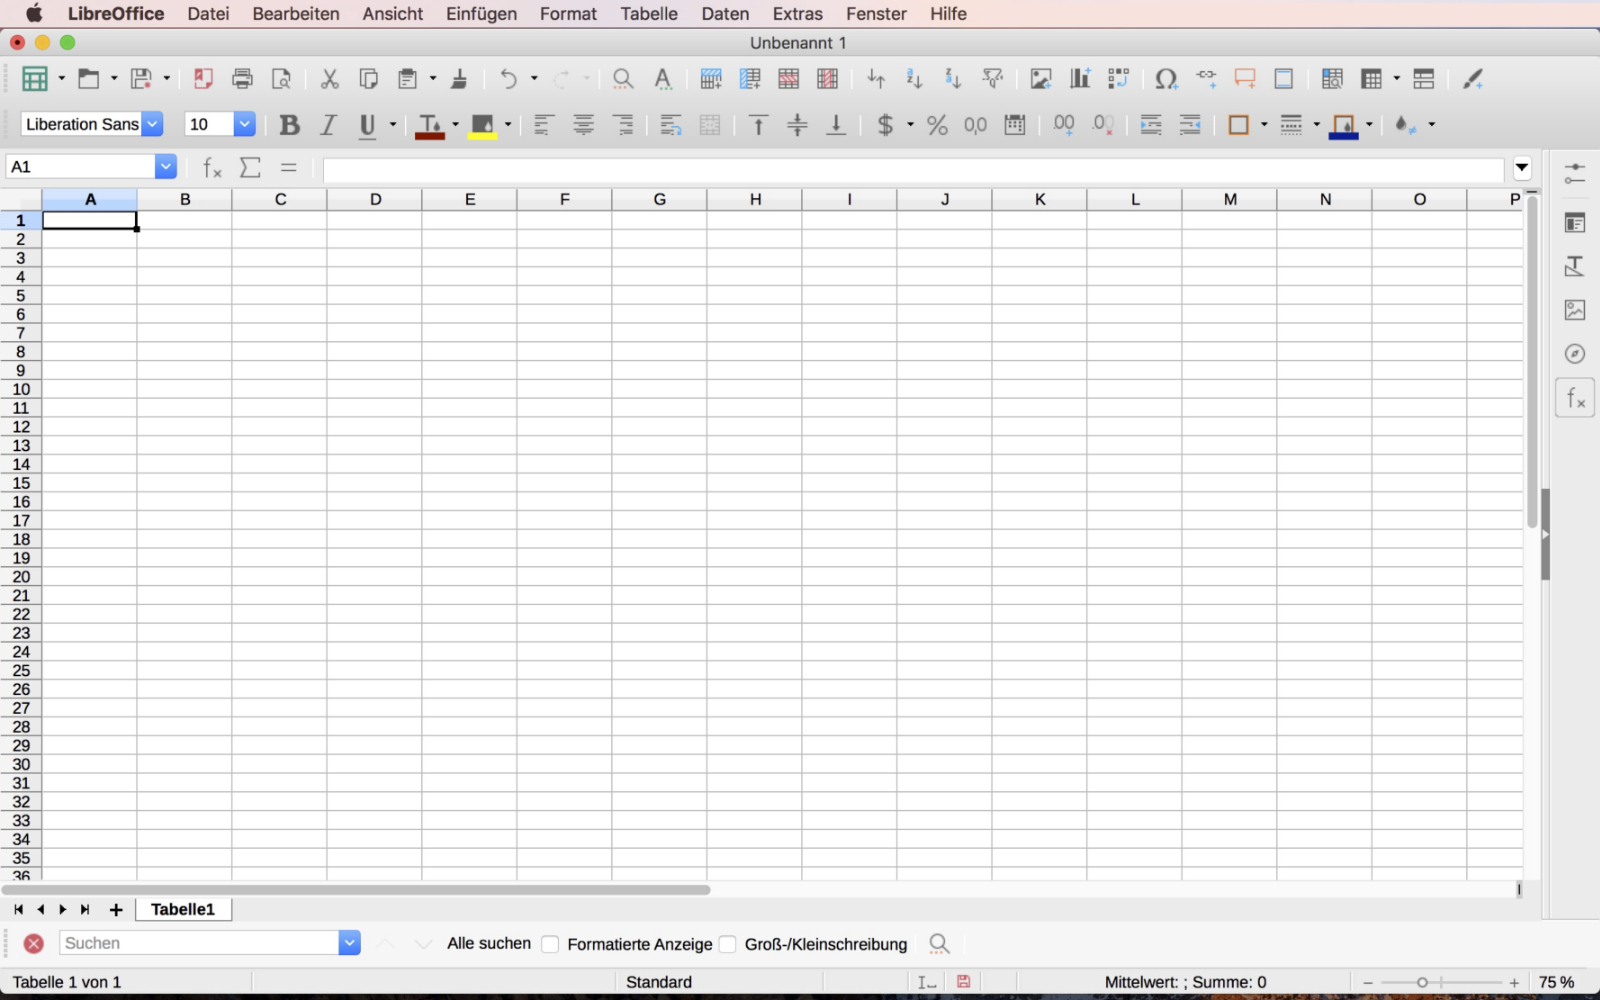
\includegraphics[width=0.9\textwidth]{img/Bildschirmfoto_mitKasten/1_Importieren_Macro/1.jpg}
		\end{figure}
	\end{onlyenv}
	\begin{onlyenv}<2>
		\begin{figure}[htbp]
			\centering
			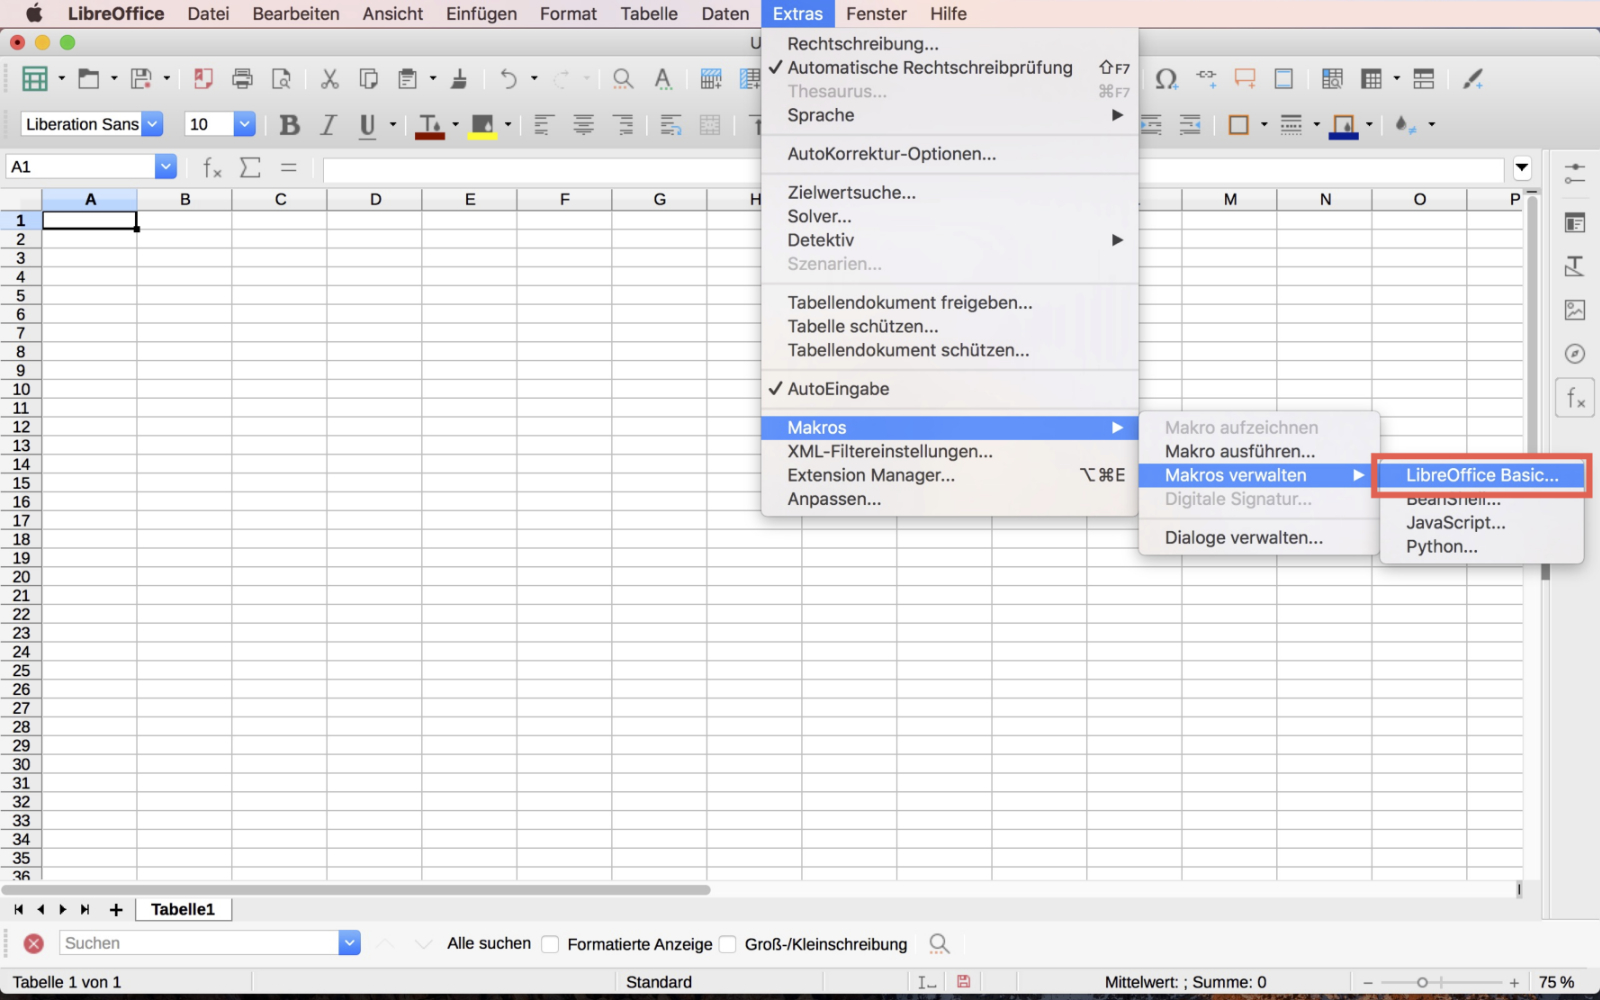
\includegraphics[width=0.9\textwidth]{img/Bildschirmfoto_mitKasten/1_Importieren_Macro/2.jpg}
		\end{figure}
	\end{onlyenv}
	\begin{onlyenv}<3>
		\begin{figure}[htbp]
			\centering
			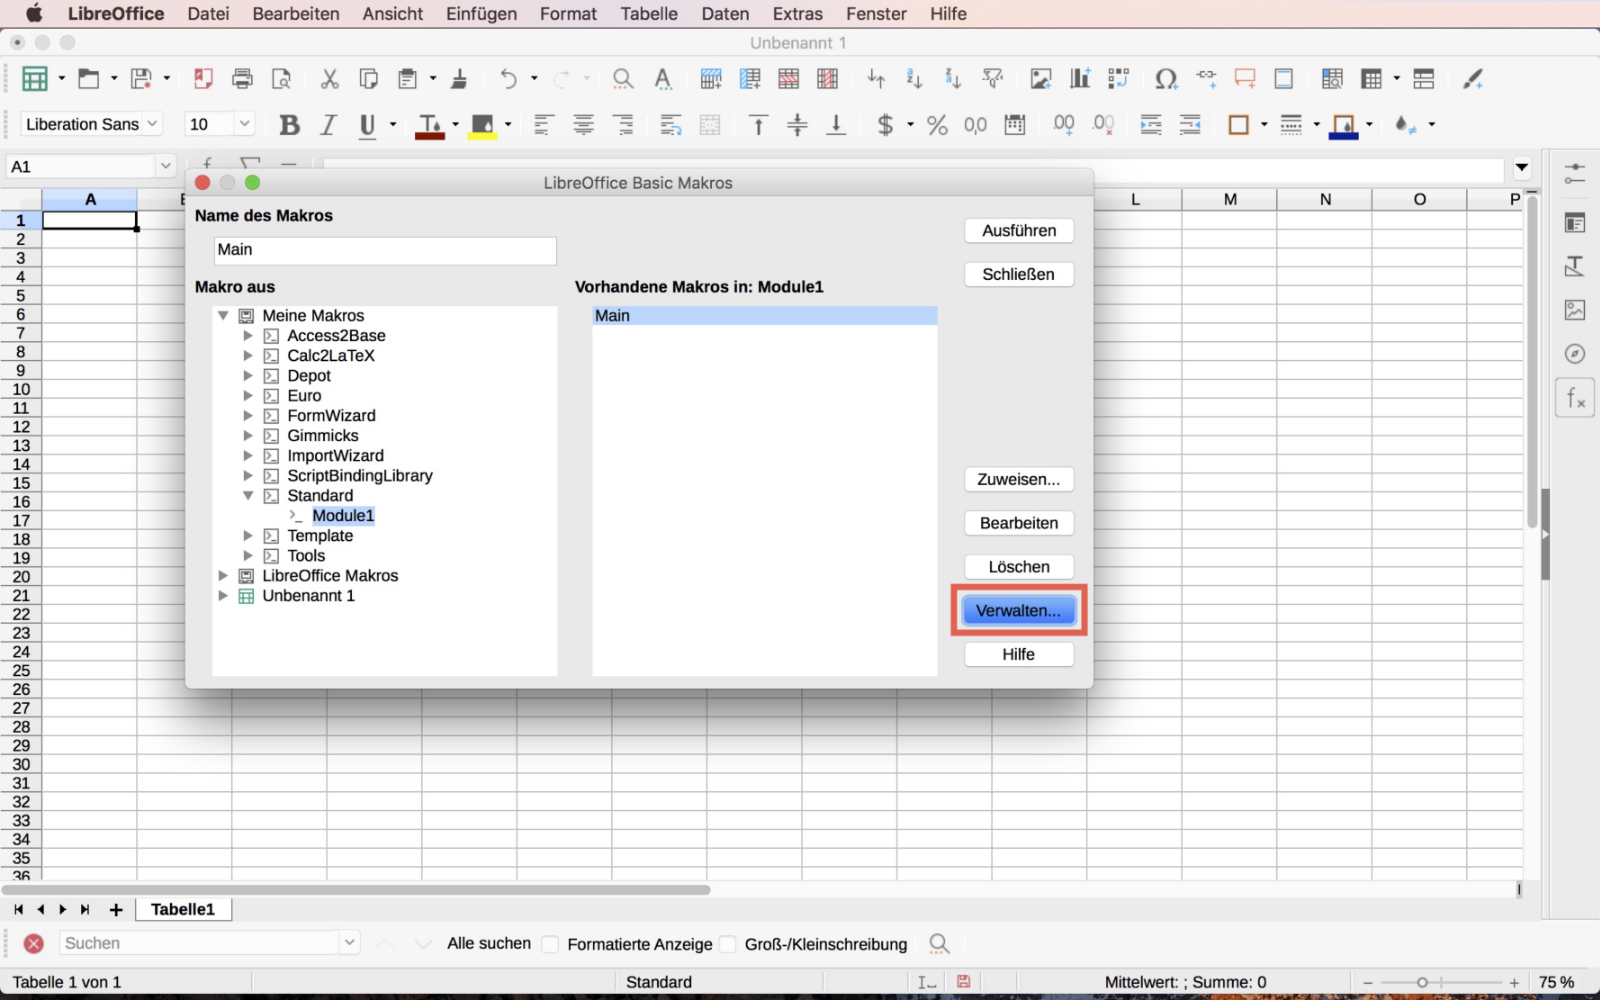
\includegraphics[width=0.9\textwidth]{img/Bildschirmfoto_mitKasten/1_Importieren_Macro/3.jpg}
		\end{figure}
	\end{onlyenv}
	\begin{onlyenv}<4>
		\begin{figure}[htbp]
			\centering
			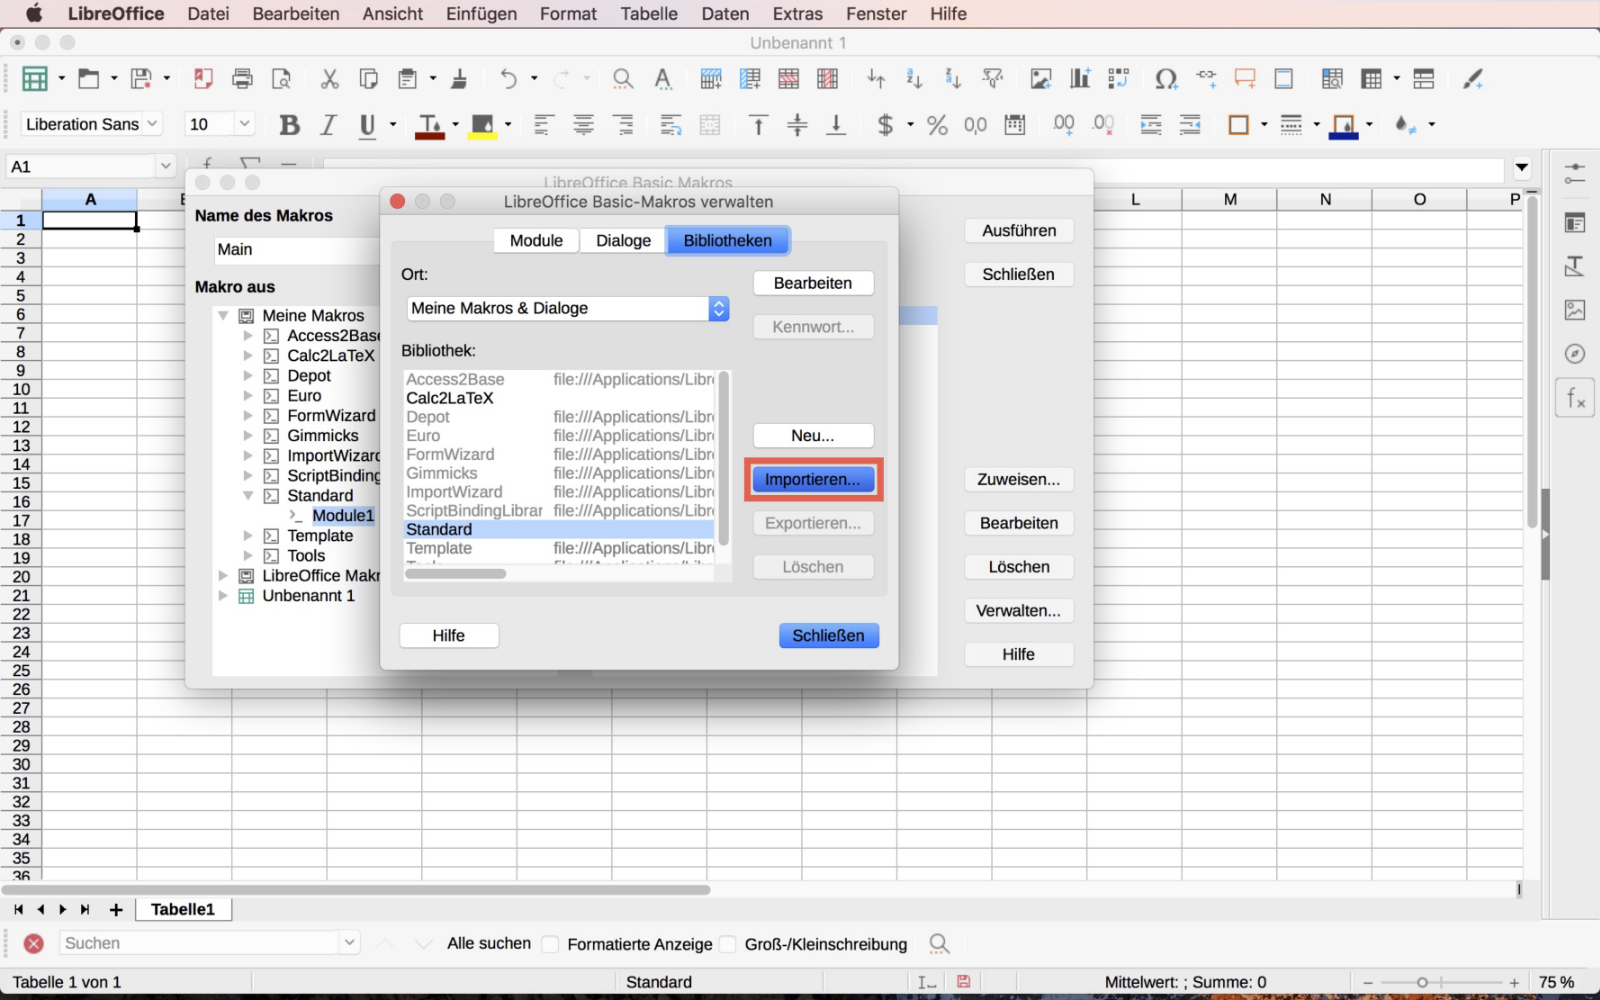
\includegraphics[width=0.9\textwidth]{img/Bildschirmfoto_mitKasten/1_Importieren_Macro/4.jpg}
		\end{figure}
	\end{onlyenv}
	\begin{onlyenv}<5>
		\begin{figure}[htbp]
			\centering
			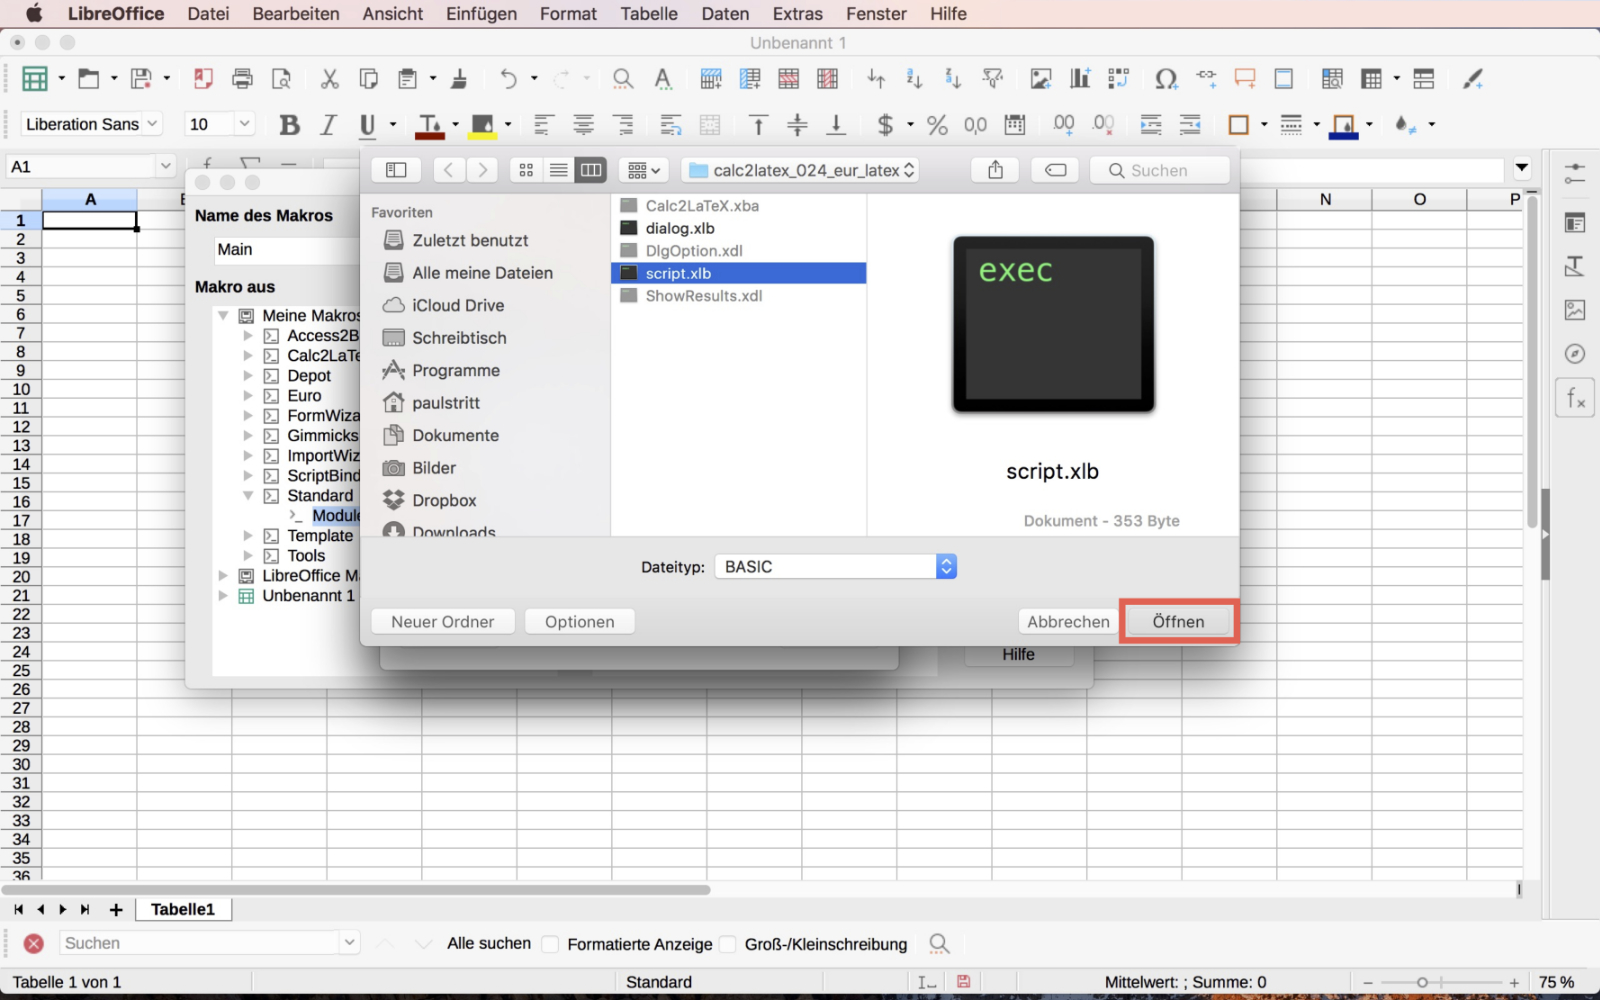
\includegraphics[width=0.9\textwidth]{img/Bildschirmfoto_mitKasten/1_Importieren_Macro/5.jpg}
		\end{figure}
	\end{onlyenv}
	\begin{onlyenv}<6>
		\begin{figure}[htbp]
			\centering
			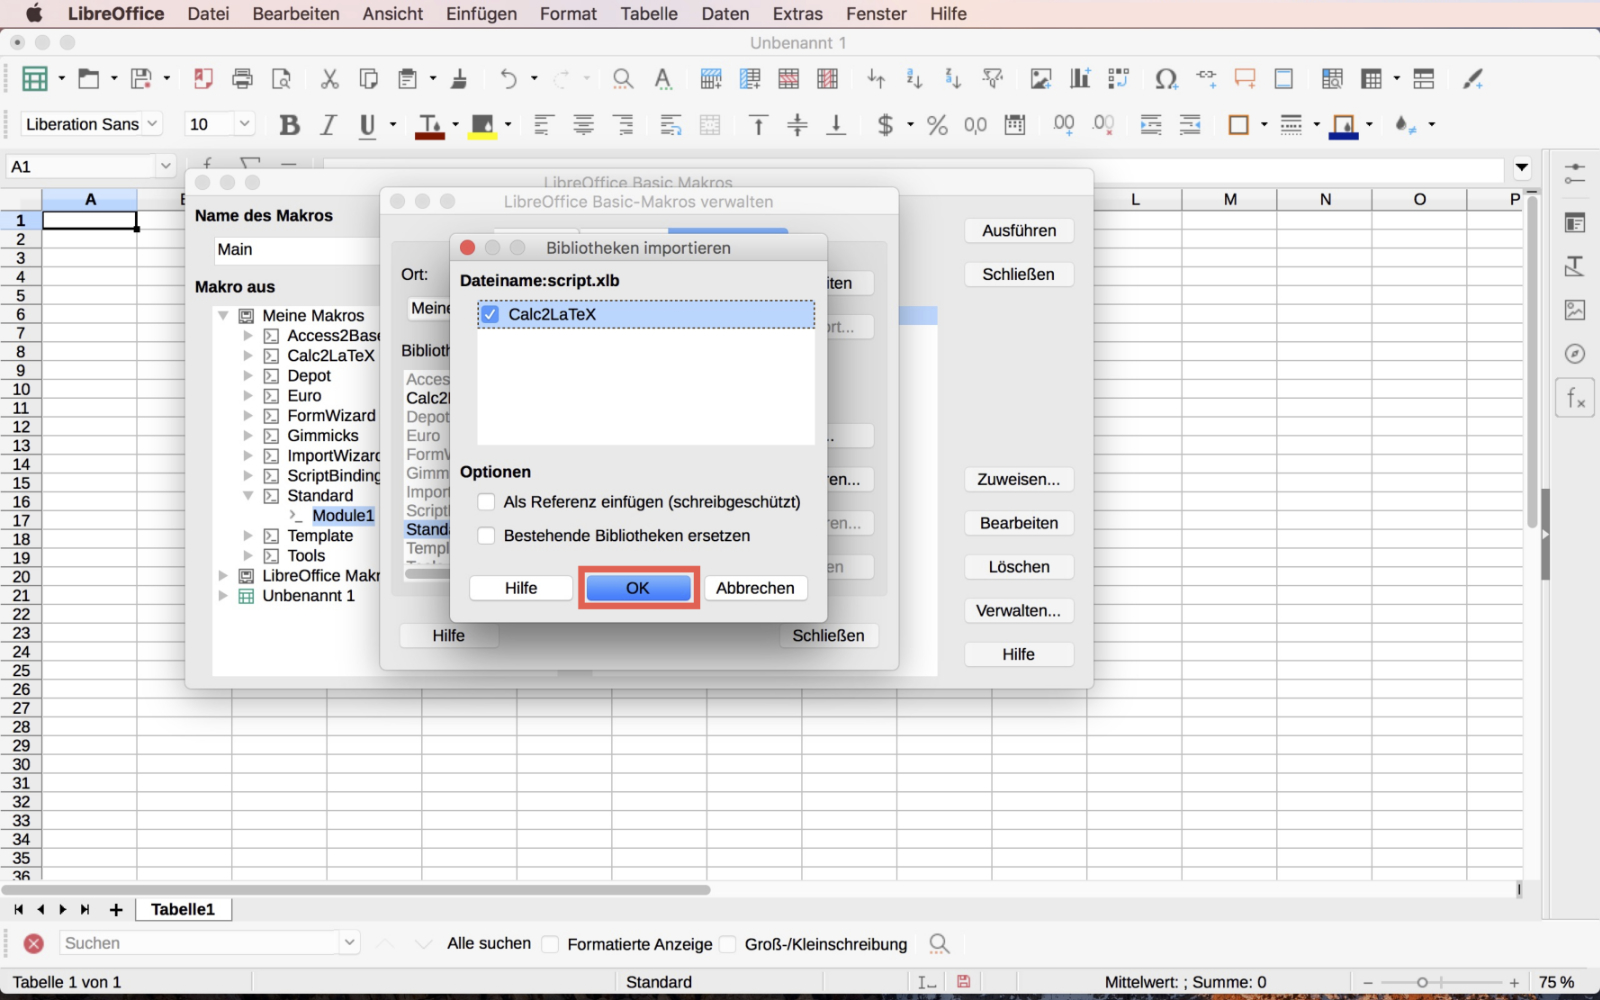
\includegraphics[width=0.9\textwidth]{img/Bildschirmfoto_mitKasten/1_Importieren_Macro/6.jpg}
		\end{figure}
	\end{onlyenv}
\end{frame}
%-----------------------------------------------------------------------------------%
%---------------------------------------FRAME---------------------------------------%
%-----------------------------------------------------------------------------------%
\begin{frame}[c]{Erstellen einer Tastenkombination für calc2latex}
	\begin{onlyenv}<1>
		\begin{figure}[htbp]
			\centering
			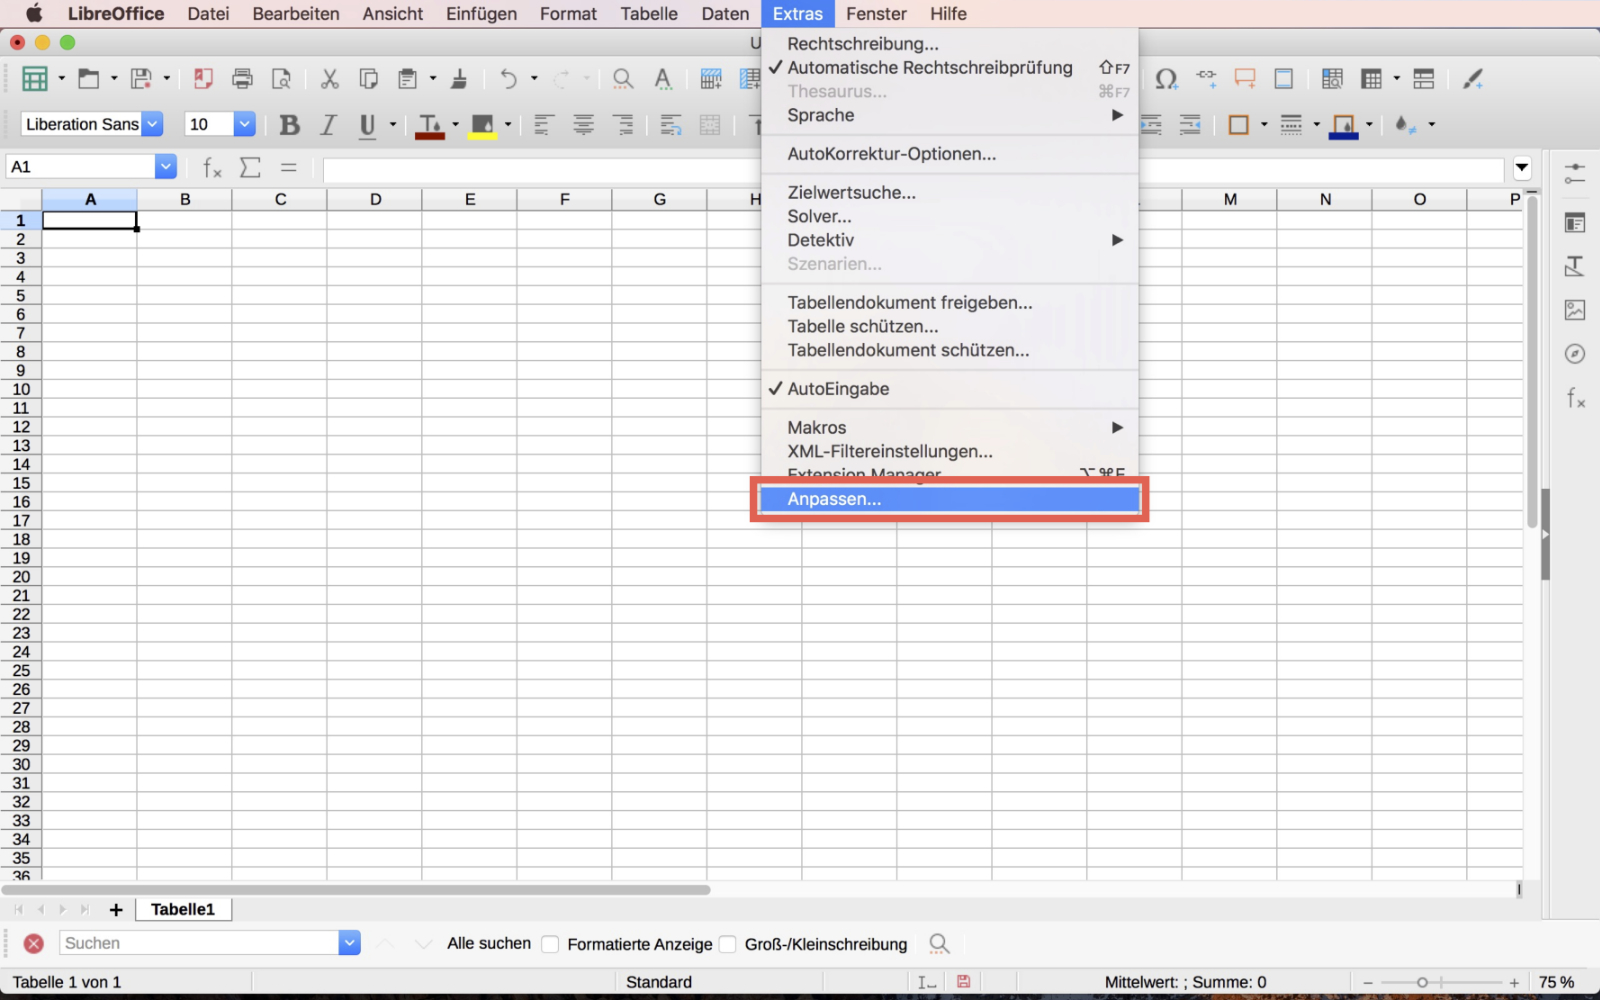
\includegraphics[width=0.9\textwidth]{img/Bildschirmfoto_mitKasten/2_Tastenkombination/1.jpg}
		\end{figure}
	\end{onlyenv}
	\begin{onlyenv}<2>
		\begin{figure}[htbp]
			\centering
			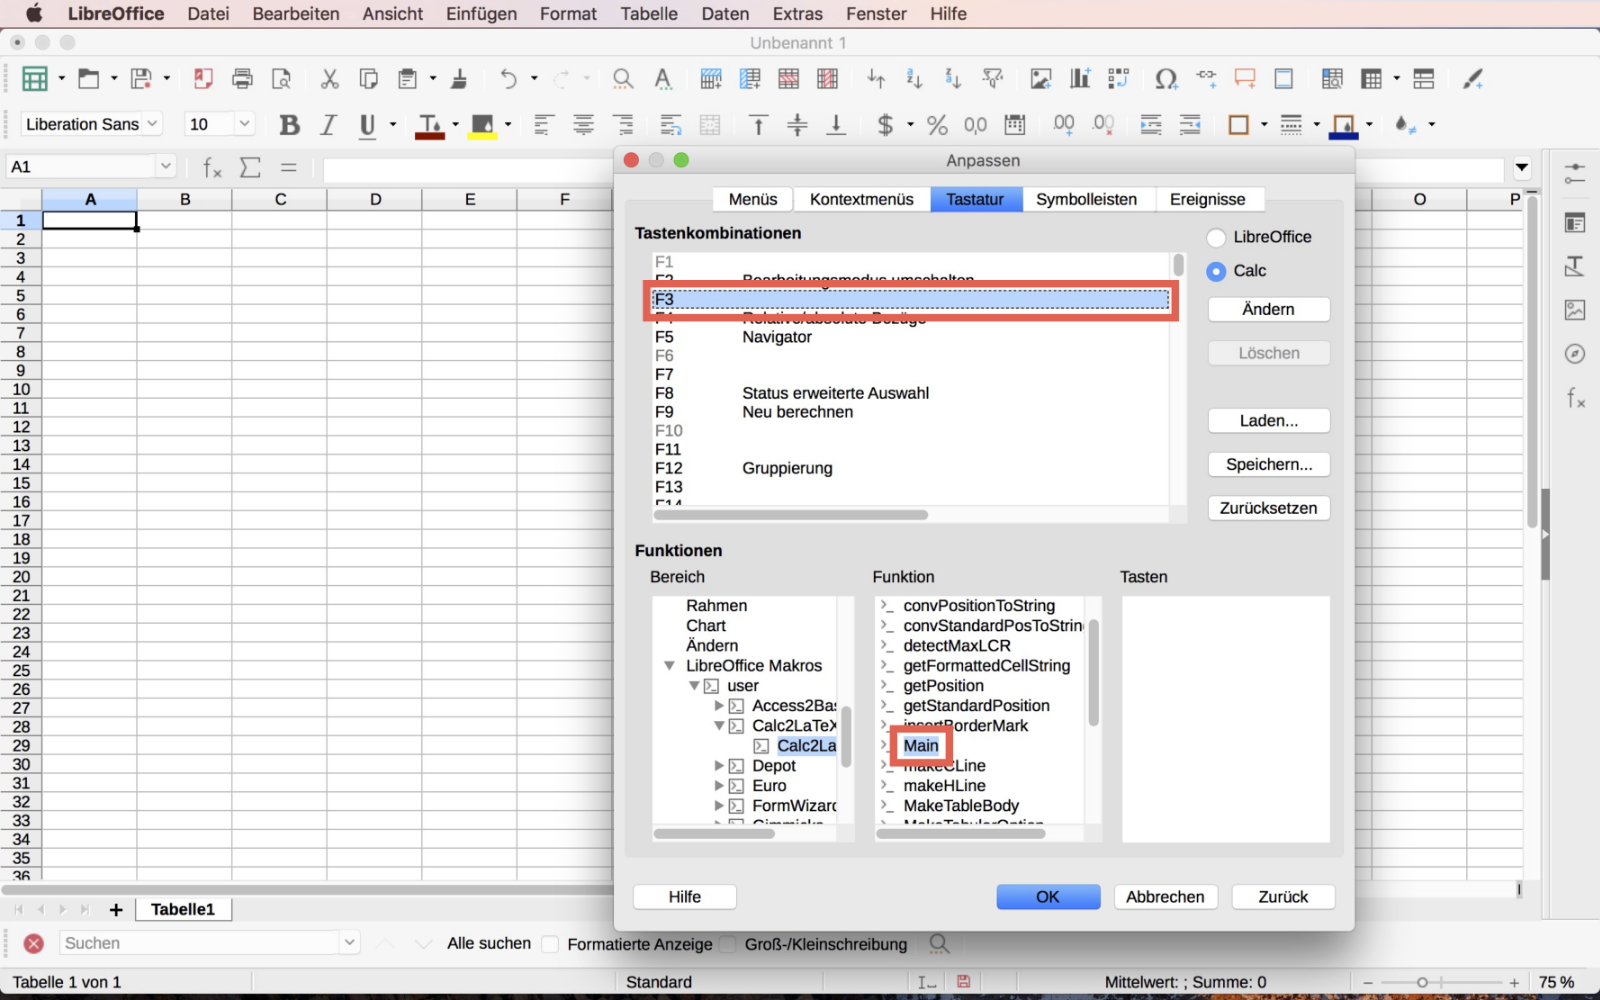
\includegraphics[width=0.9\textwidth]{img/Bildschirmfoto_mitKasten/2_Tastenkombination/2.jpg}
		\end{figure}
	\end{onlyenv}
	\begin{onlyenv}<3>
		\begin{figure}[htbp]
			\centering
			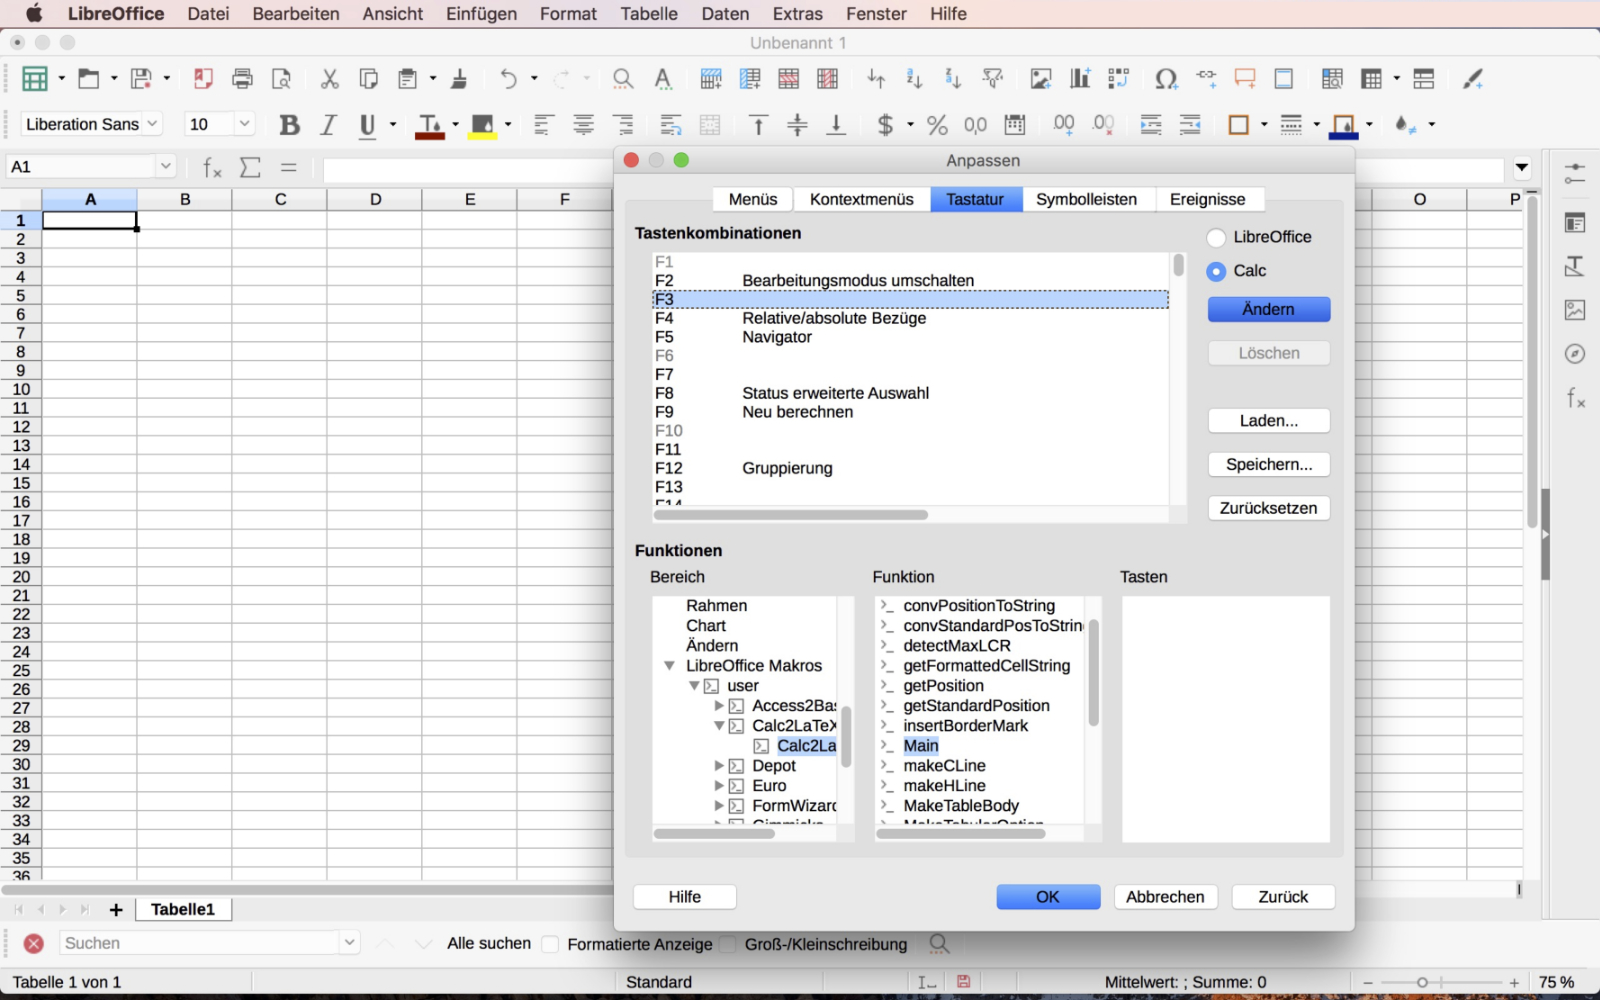
\includegraphics[width=0.9\textwidth]{img/Bildschirmfoto_mitKasten/2_Tastenkombination/3.jpg}
		\end{figure}
	\end{onlyenv}
	\begin{onlyenv}<4>
		\begin{figure}[htbp]
			\centering
			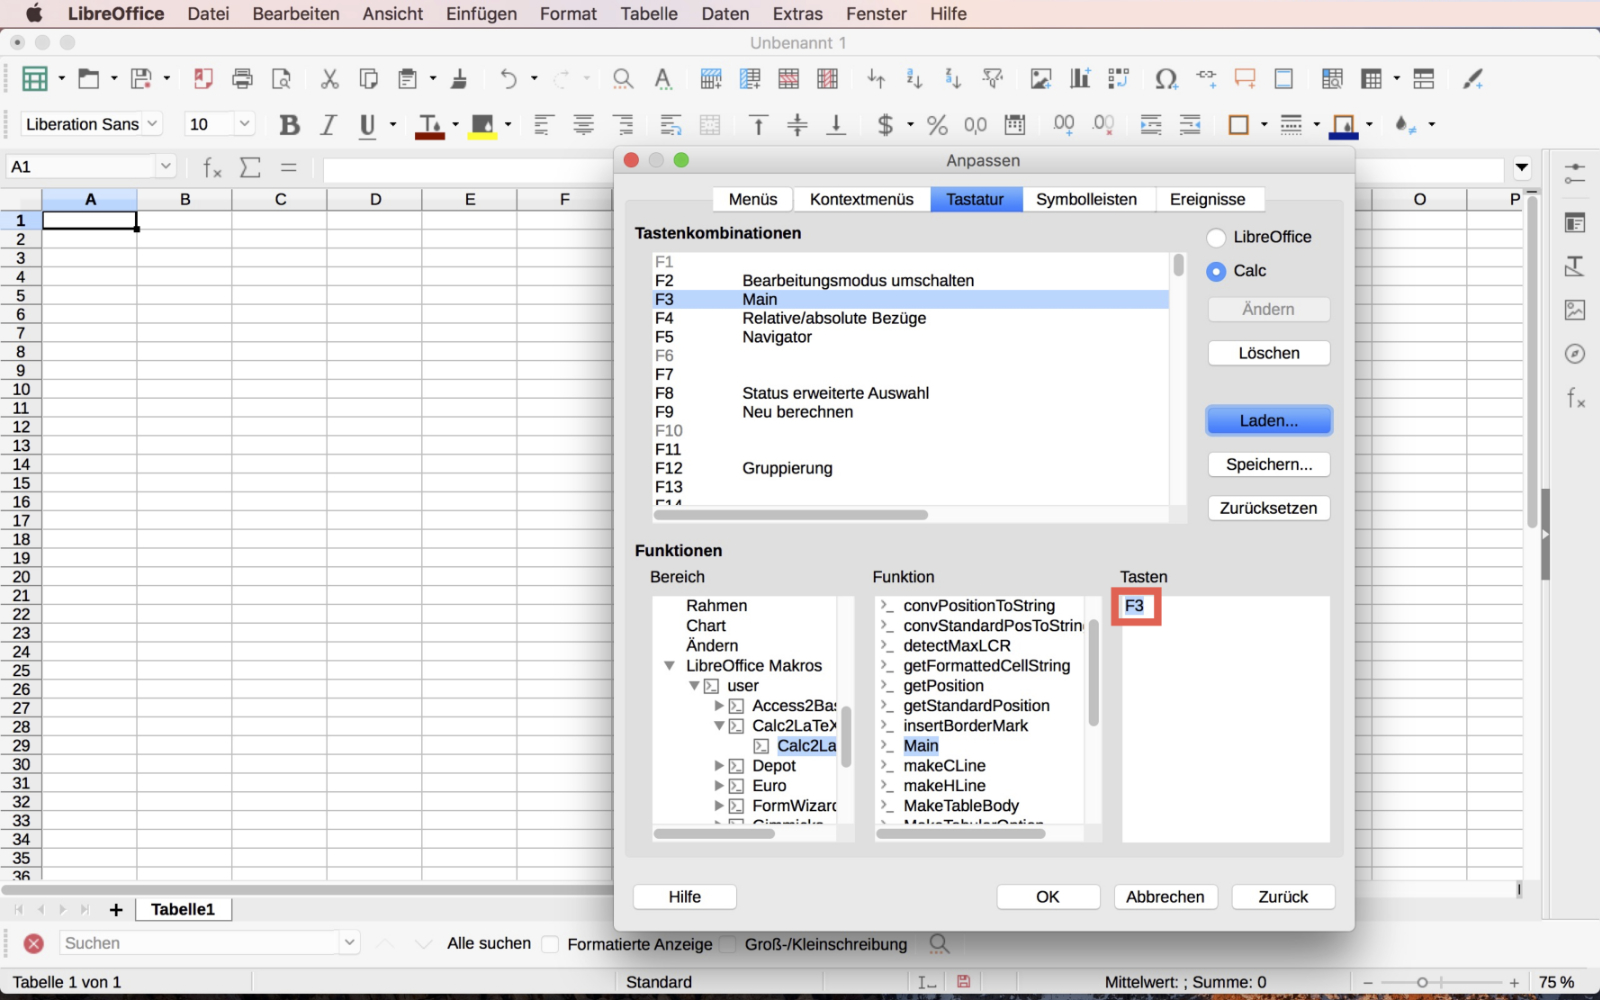
\includegraphics[width=0.9\textwidth]{img/Bildschirmfoto_mitKasten/2_Tastenkombination/4.jpg}
		\end{figure}
	\end{onlyenv}
\end{frame}
%-----------------------------------------------------------------------------------%
%---------------------------------------FRAME---------------------------------------%
%-----------------------------------------------------------------------------------%
\begin{frame}[c]{Erstellen der Tabelle}
	\begin{onlyenv}<1>
		\begin{figure}[htbp]
			\centering
			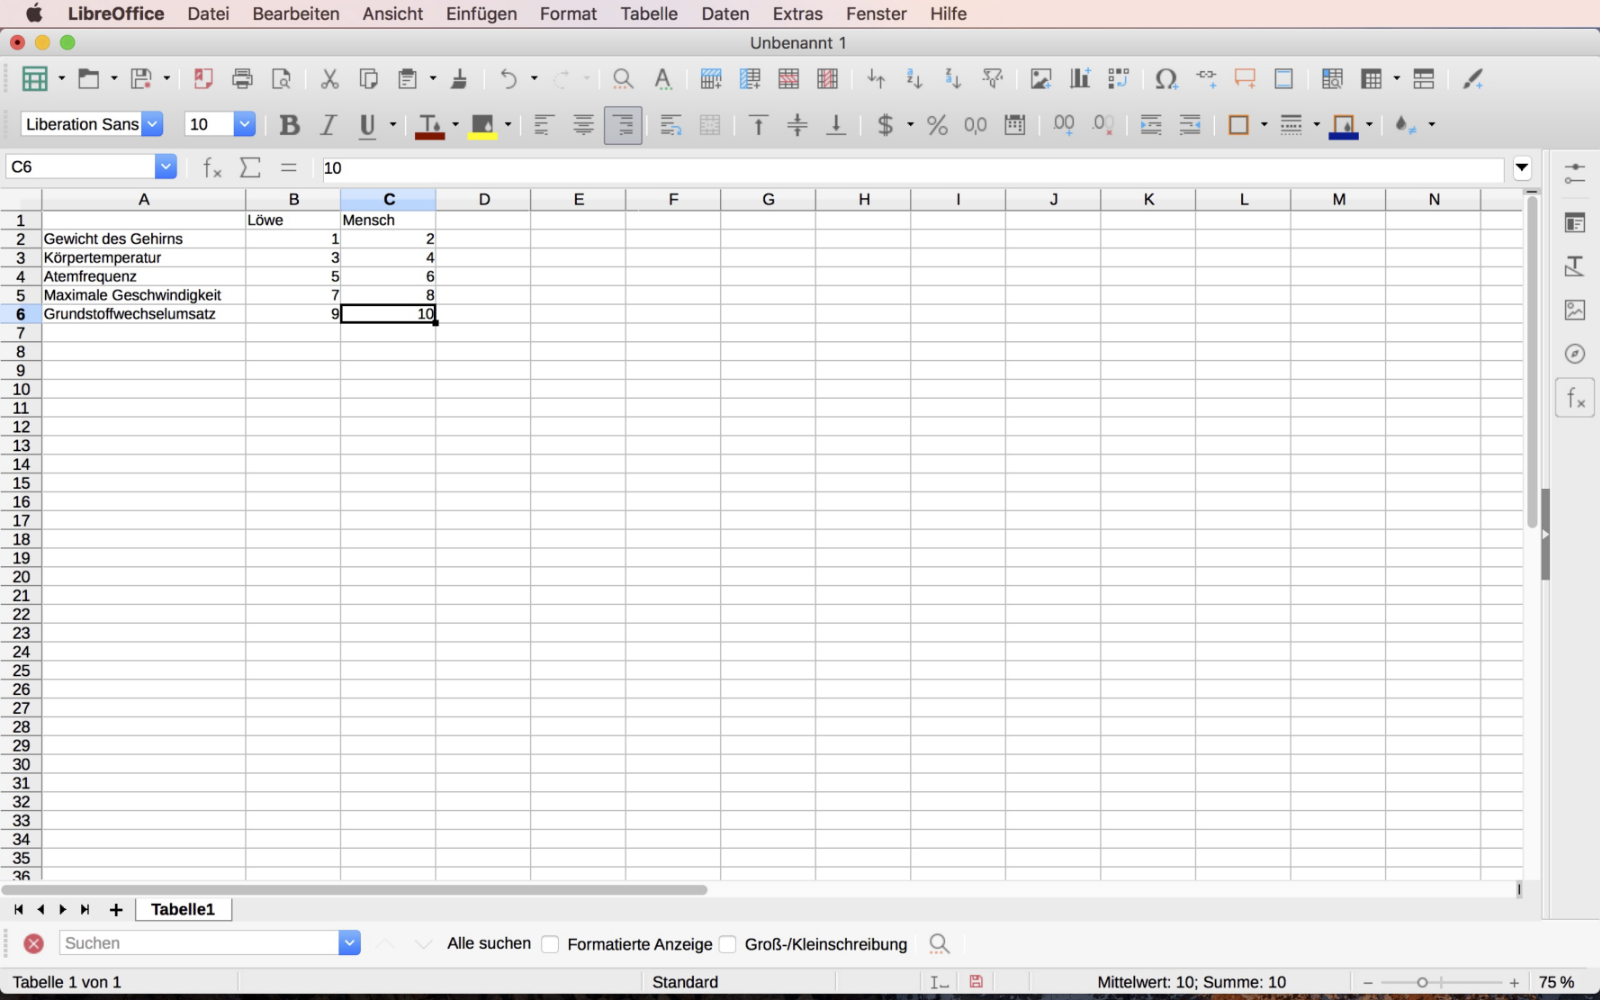
\includegraphics[width=0.9\textwidth]{img/Bildschirmfoto_mitKasten/3_Tabelle/1.jpg}
		\end{figure}
	\end{onlyenv}
	\begin{onlyenv}<2>
		\begin{figure}[htbp]
			\centering
			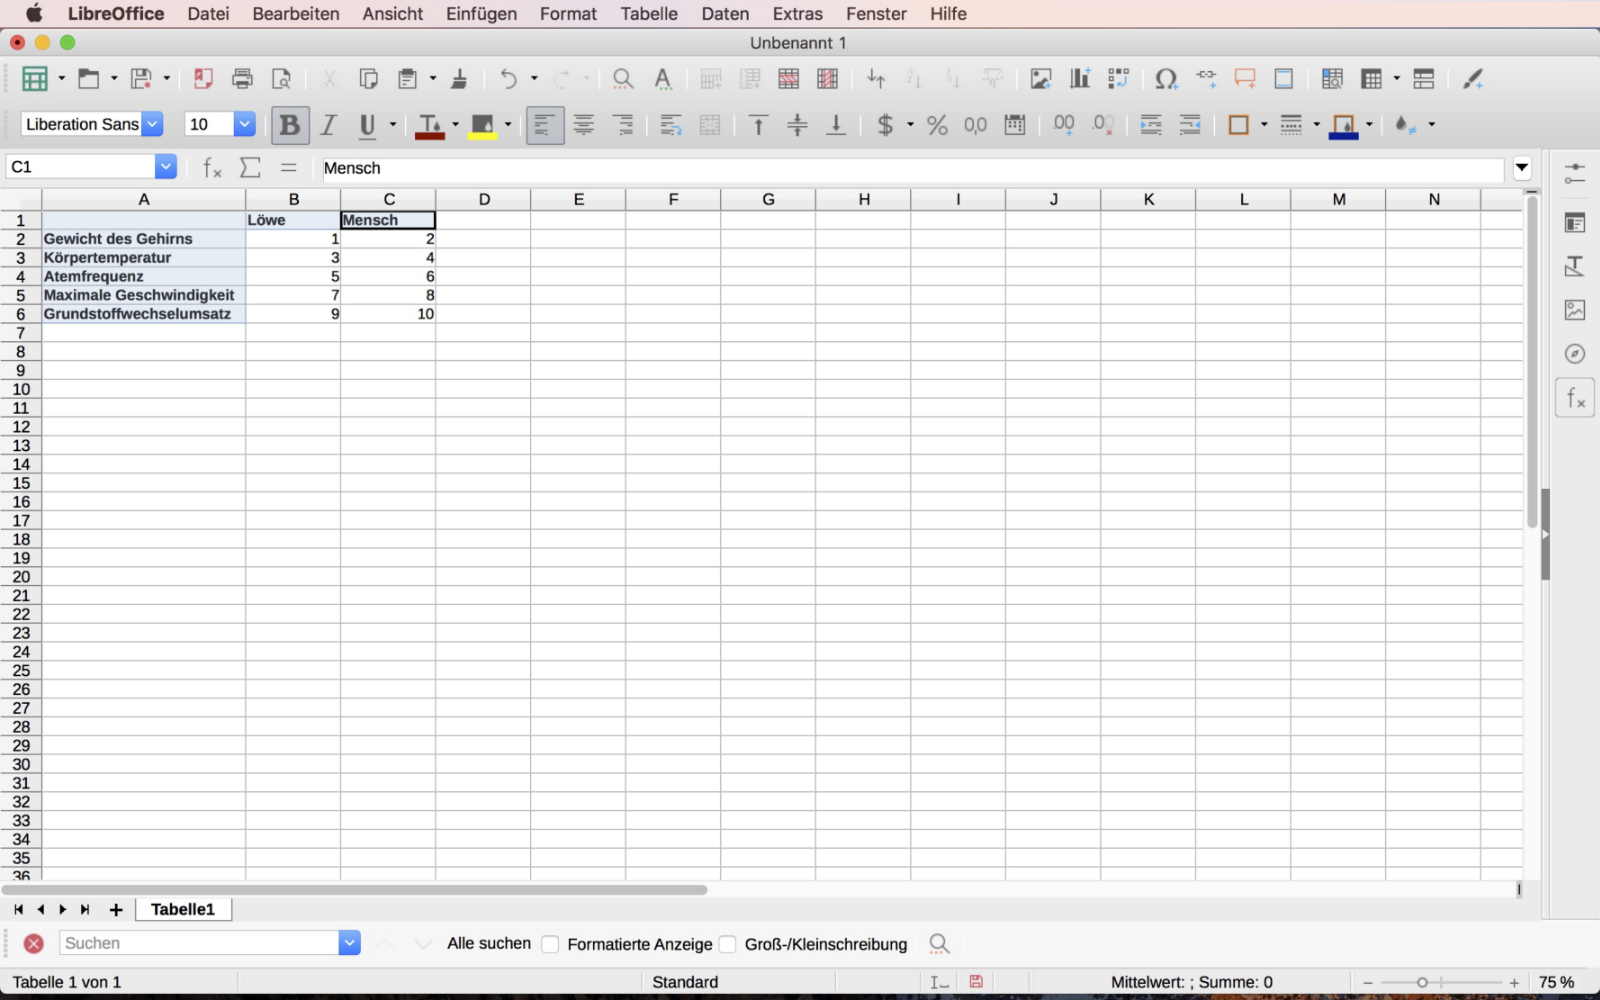
\includegraphics[width=0.9\textwidth]{img/Bildschirmfoto_mitKasten/3_Tabelle/2.jpg}
		\end{figure}
	\end{onlyenv}
	\begin{onlyenv}<3>
		\begin{figure}[htbp]
			\centering
			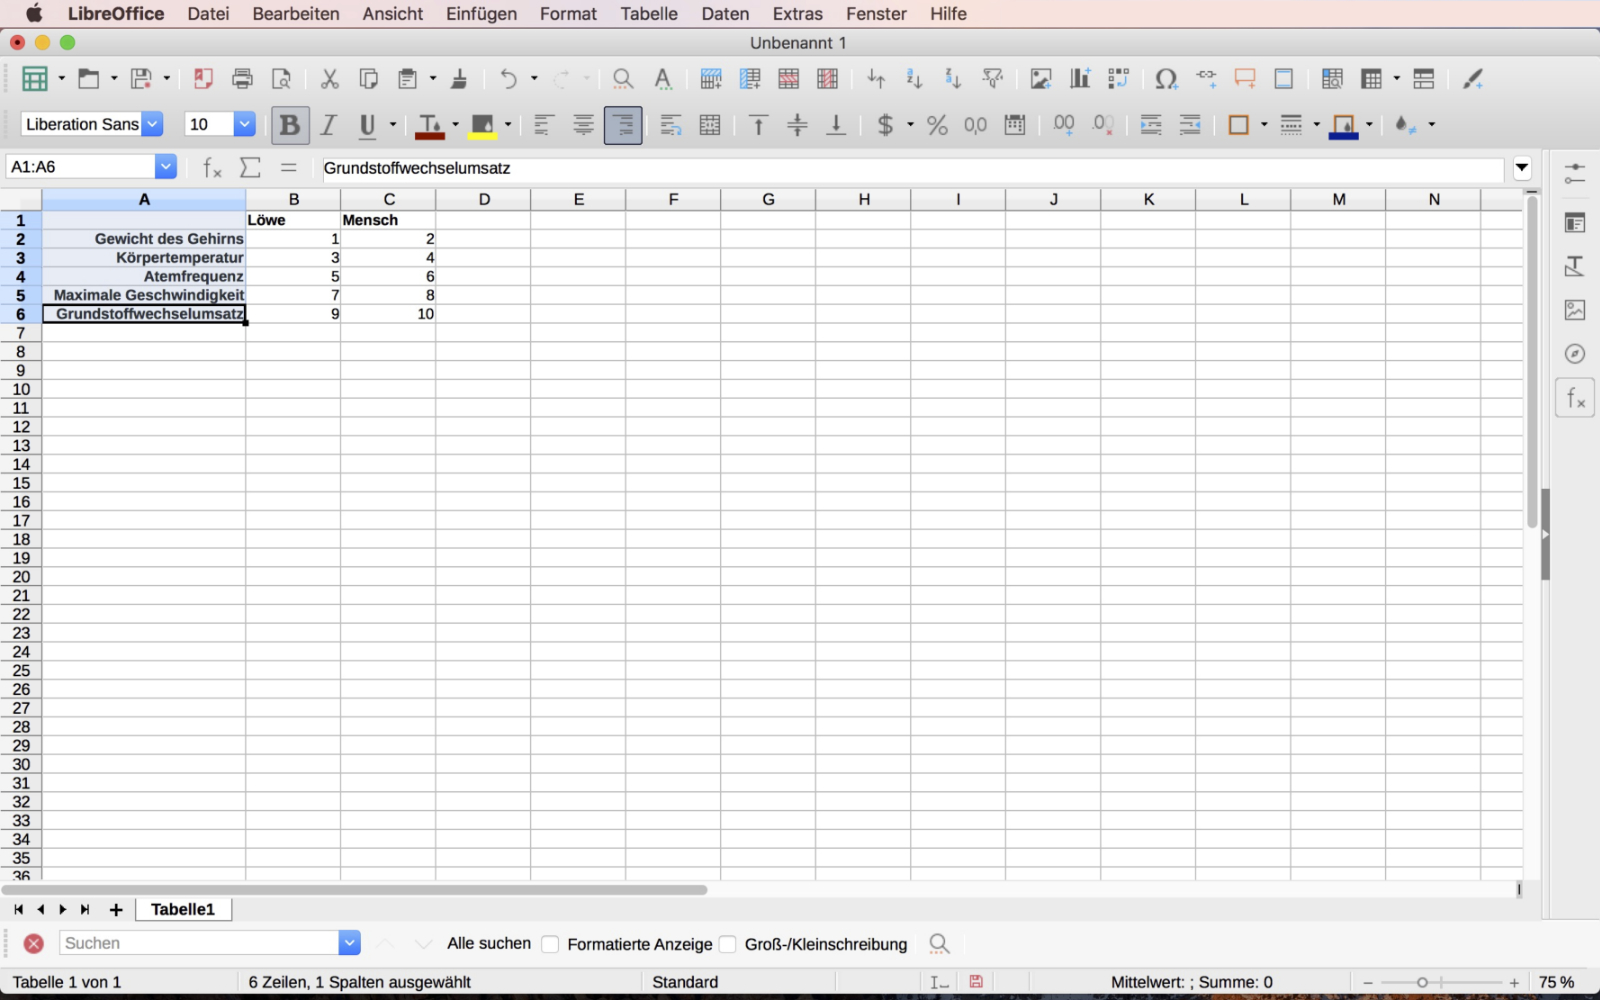
\includegraphics[width=0.9\textwidth]{img/Bildschirmfoto_mitKasten/3_Tabelle/3.jpg}
		\end{figure}
	\end{onlyenv}
	\begin{onlyenv}<4>
		\begin{figure}[htbp]
			\centering
			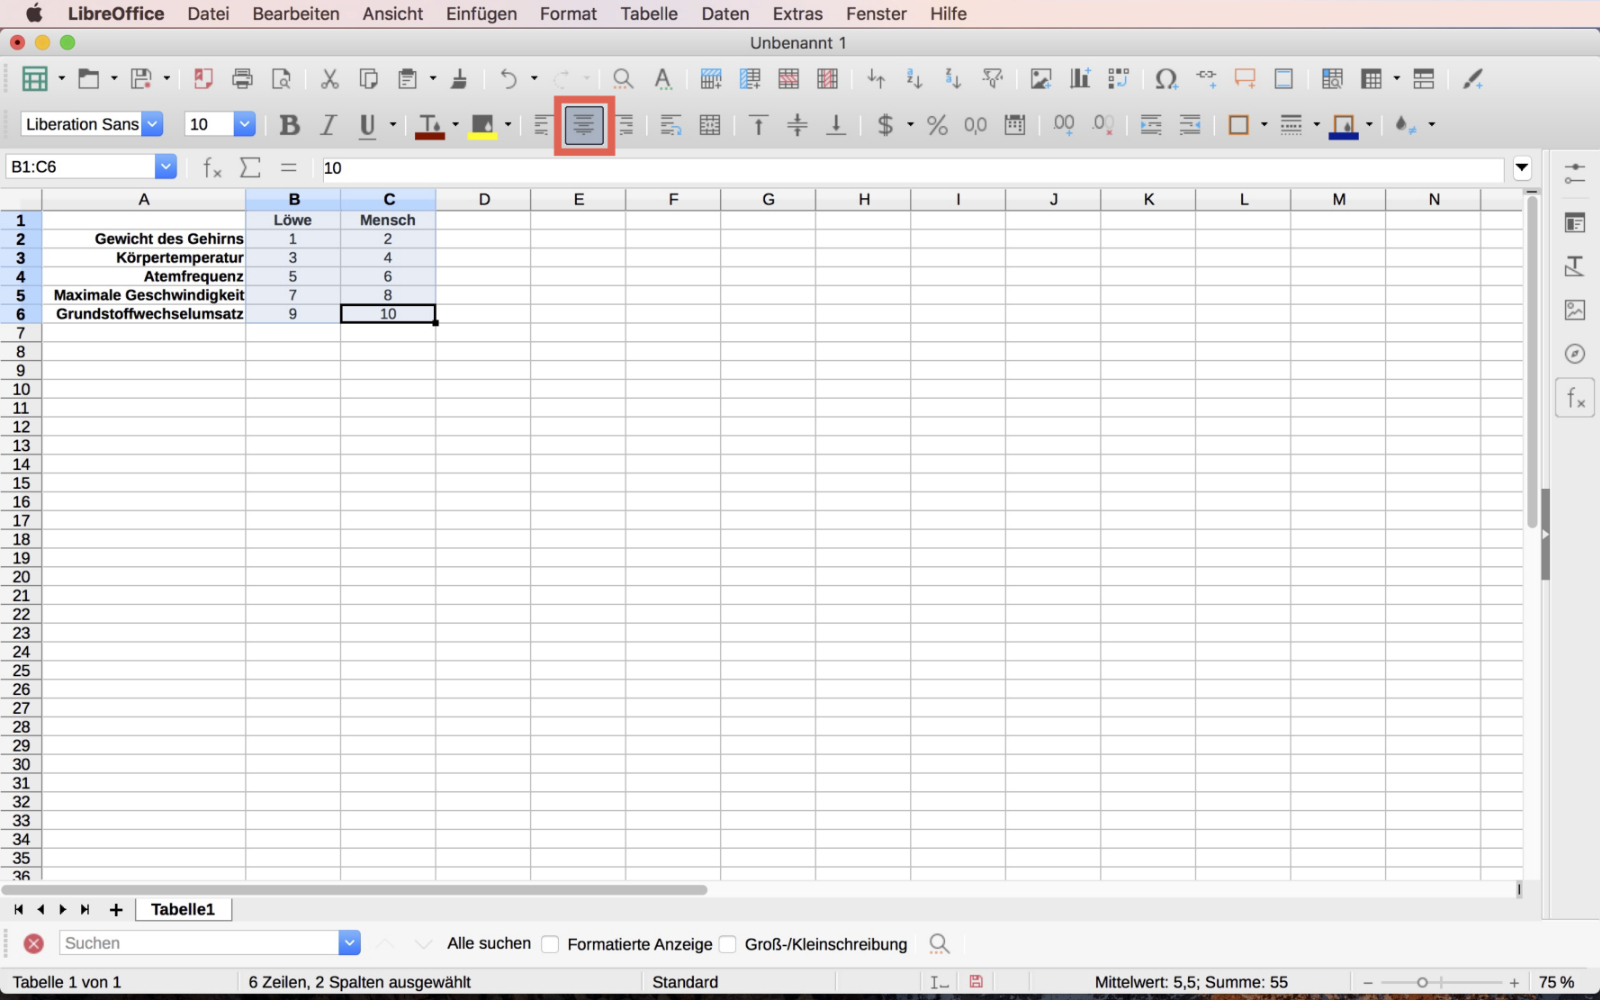
\includegraphics[width=0.9\textwidth]{img/Bildschirmfoto_mitKasten/3_Tabelle/4.jpg}
		\end{figure}
	\end{onlyenv}
	\begin{onlyenv}<5>
		\begin{figure}[htbp]
			\centering
			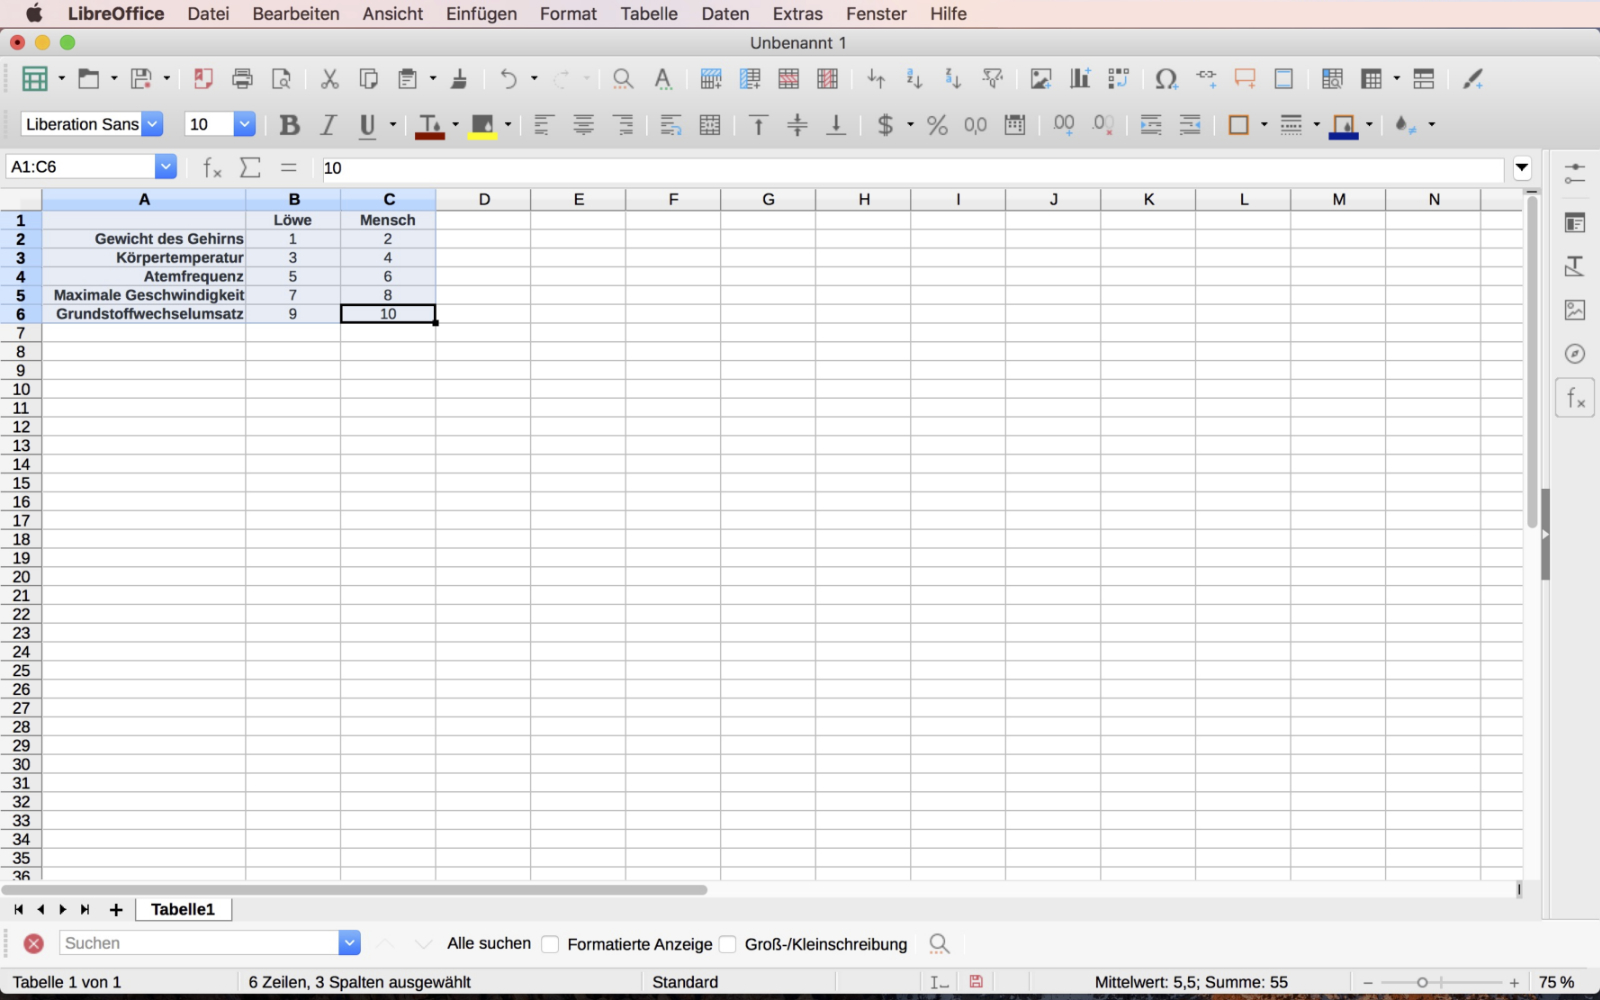
\includegraphics[width=0.9\textwidth]{img/Bildschirmfoto_mitKasten/3_Tabelle/5.jpg}
		\end{figure}
	\end{onlyenv}
\end{frame}
%-----------------------------------------------------------------------------------%
%---------------------------------------FRAME---------------------------------------%
%-----------------------------------------------------------------------------------%
\begin{frame}[c]{Ausführen des Makros}
	\begin{onlyenv}<1>
		\begin{figure}[htbp]
			\centering
			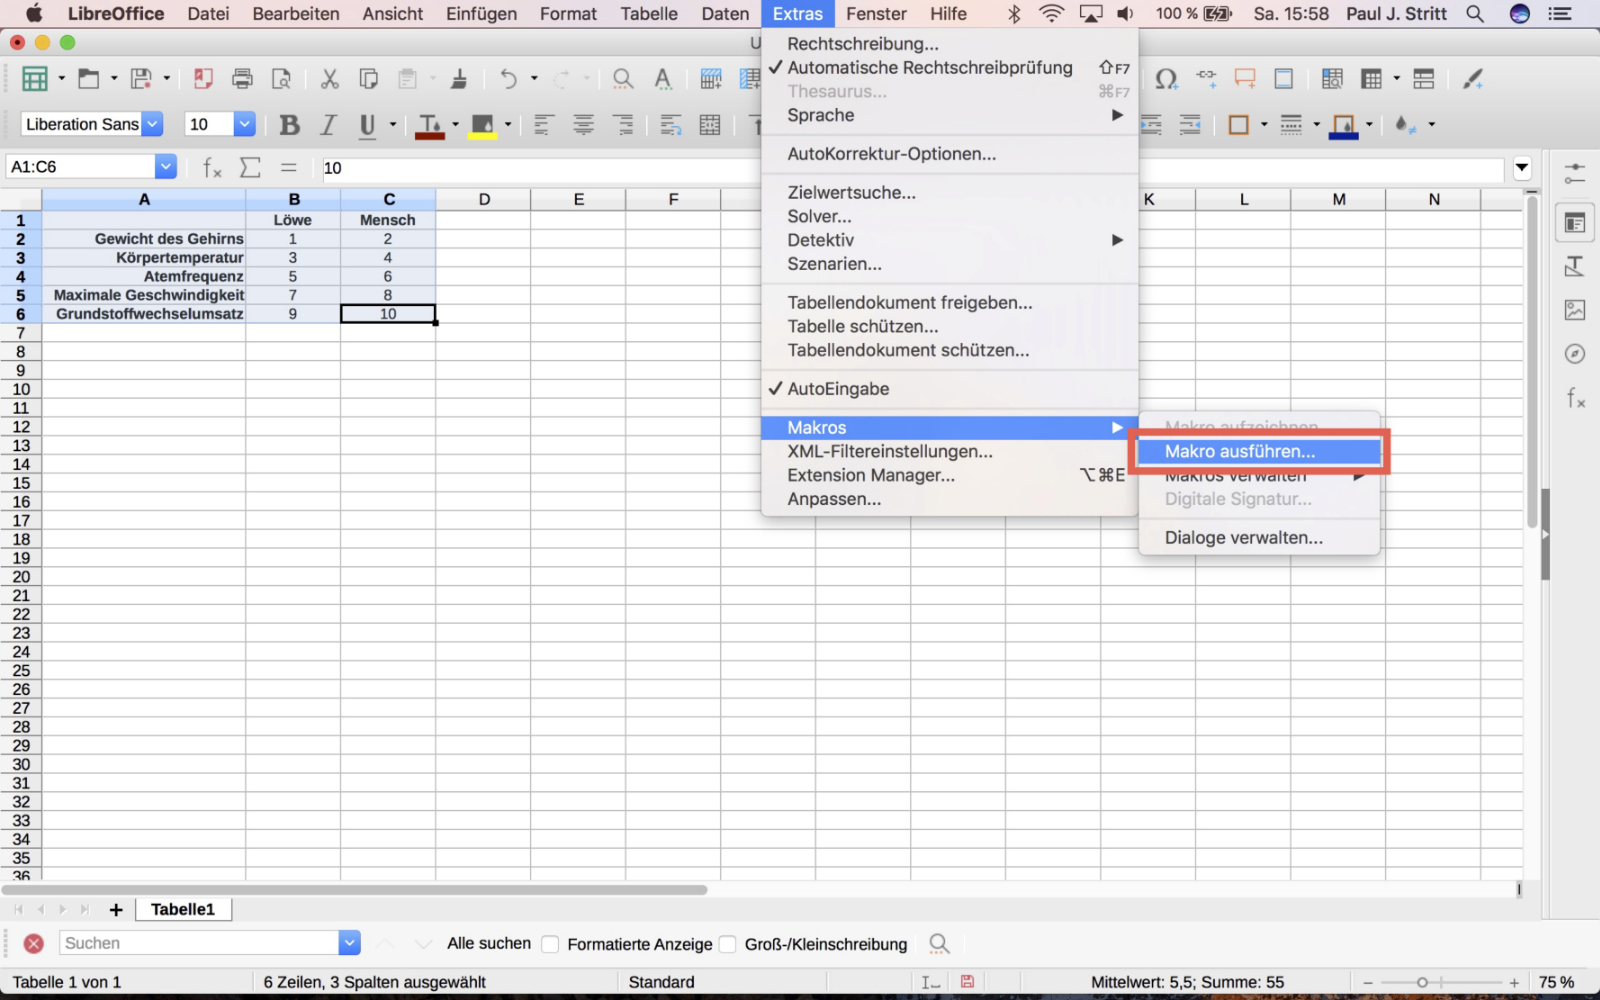
\includegraphics[width=0.9\textwidth]{img/Bildschirmfoto_mitKasten/4_Ausfuhren_Macro/1.jpg}
		\end{figure}
	\end{onlyenv}
	\begin{onlyenv}<2>
		\begin{figure}[htbp]
			\centering
			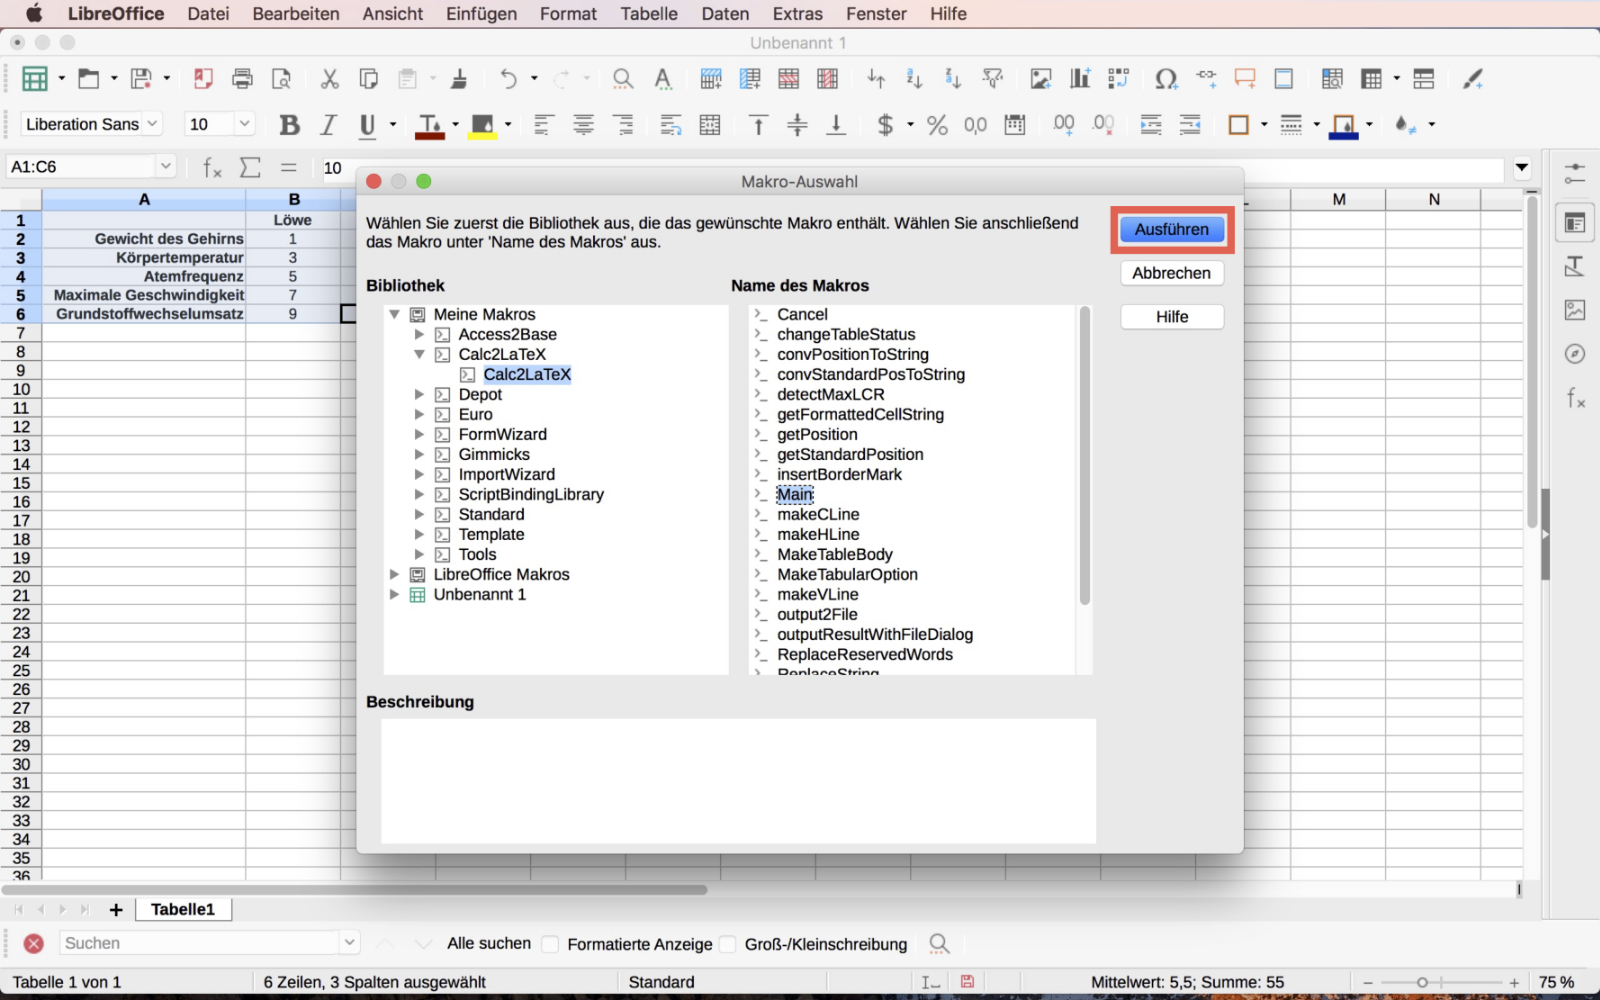
\includegraphics[width=0.9\textwidth]{img/Bildschirmfoto_mitKasten/4_Ausfuhren_Macro/2.jpg}
		\end{figure}
	\end{onlyenv}
	\begin{onlyenv}<3>
		\begin{figure}[htbp]
			\centering
			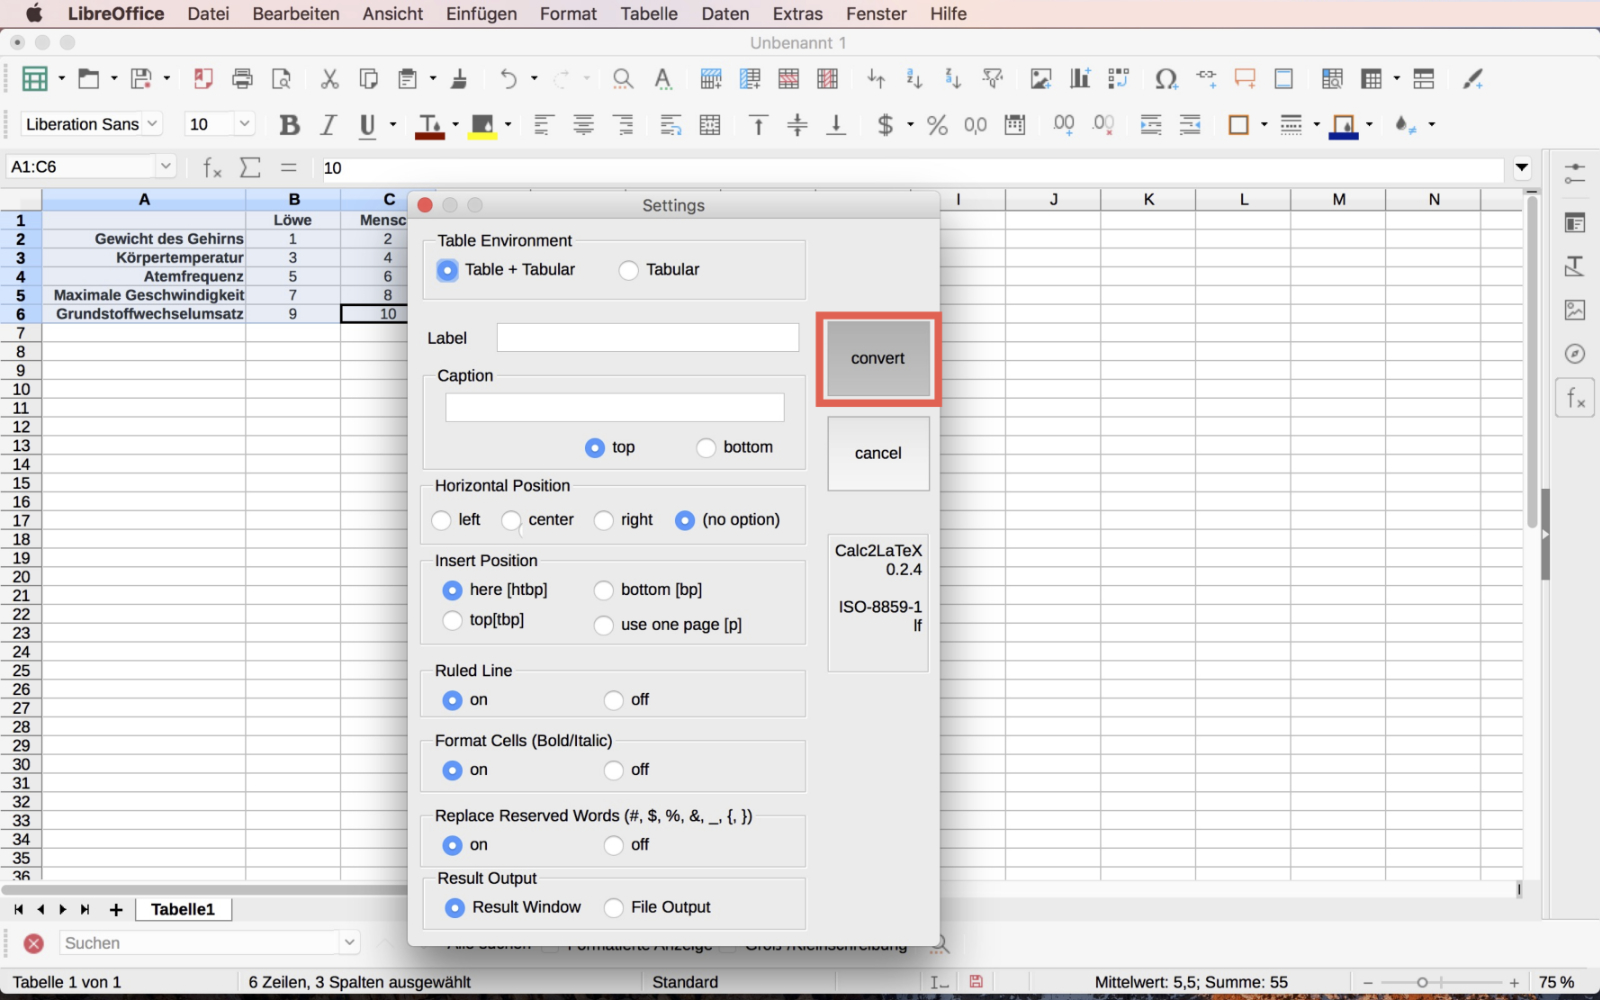
\includegraphics[width=0.9\textwidth]{img/Bildschirmfoto_mitKasten/3_Tabelle/6.jpg}
		\end{figure}
	\end{onlyenv}
	\begin{onlyenv}<4>
		\begin{figure}[htbp]
			\centering
			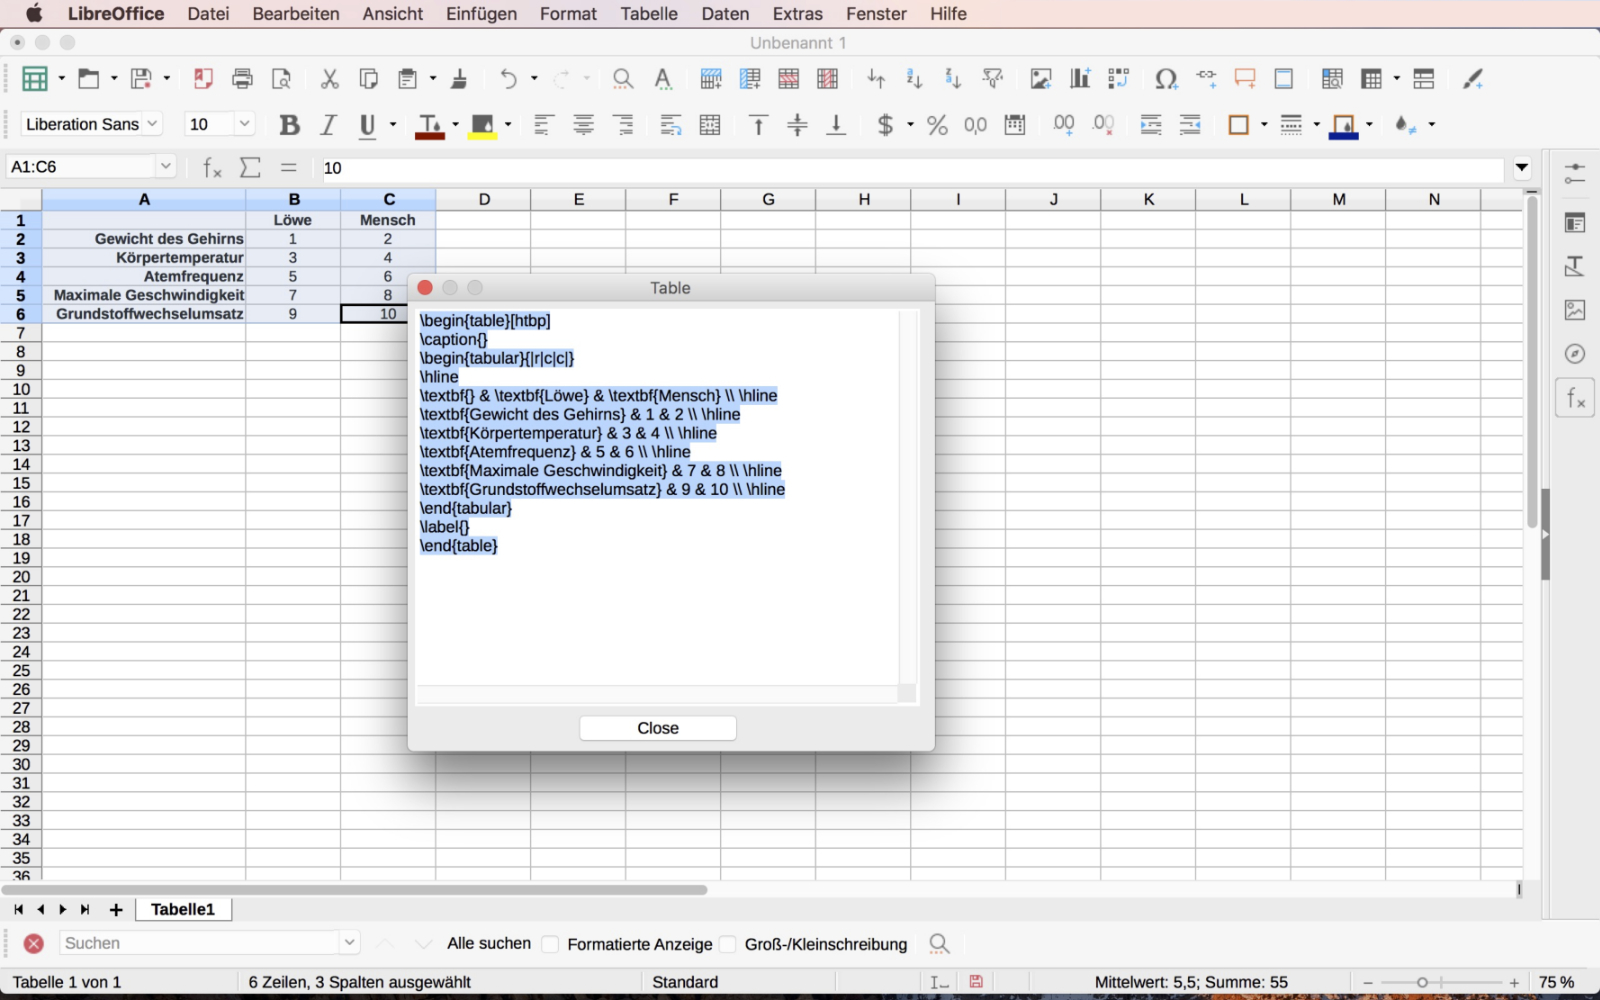
\includegraphics[width=0.9\textwidth]{img/Bildschirmfoto_mitKasten/3_Tabelle/7.jpg}
		\end{figure}
	\end{onlyenv}
\end{frame}
%-----------------------------------------------------------------------------------%
%---------------------------------------FRAME---------------------------------------%
%-----------------------------------------------------------------------------------%
\begin{frame}[fragile]
	\begin{onlyenv}<1>
	\Ausgabe
	\begin{outputbox}
		\begin{table}
			\centering
			\begin{tabular}{lll}
				Überschrift 1	&	Überschrift 2	&	Überschrift 3	\\
				Inhalt 1		&	Inhalt 2		&	Inhalt 3	\\
				Inhalt 4		&	Inhalt 5		&	Inhalt 6	\\
			\end{tabular}
			\end{table}
		\end{outputbox}
	\end{onlyenv}

	\begin{onlyenv}<2>
		\Code
		\begin{lstlisting}
\begin{table}
	\centering
	
\end{table}
		\end{lstlisting}
		\Ausgabe
		\begin{outputbox}
			\begin{table}
				\centering
	
			\end{table}
		\end{outputbox}
	\end{onlyenv}

	\begin{onlyenv}<3>
		\Code
		\begin{lstlisting}
\begin{table}
	\centering
	\begin{tabular}{c}
		Inhalt 1
	\end{tabular}
\end{table}
		\end{lstlisting}
		\Ausgabe
		\begin{outputbox}
			\begin{table}
				\centering
				\begin{tabular}{c}
					Inhalt 1
				\end{tabular}
			\end{table}
		\end{outputbox}
	\end{onlyenv}
	
	\begin{onlyenv}<4>
		\Code
		\begin{lstlisting}
\begin{table}
	\centering
	\begin{tabular}{ccc}
		Inhalt 1 & Inhalt 2 & Inhalt 3
	\end{tabular}
\end{table}
		\end{lstlisting}
		\Ausgabe
		\begin{outputbox}
			\begin{table}
				\centering
				\begin{tabular}{ccc}
					Inhalt 1 & Inhalt 2 & Inhalt 3
				\end{tabular}
			\end{table}
		\end{outputbox}
	\end{onlyenv}

	\begin{onlyenv}<5>
		\Code
		\begin{lstlisting}
\begin{table}
	\centering
	\begin{tabular}{ccc}
		Überschrift 1 & Überschrift 2 & Überschrift 3	\\
		Inhalt 1      & Inhalt 2      & Inhalt 3
	\end{tabular}
\end{table}
		\end{lstlisting}
		\Ausgabe
		\begin{outputbox}
			\begin{table}
				\centering
				\begin{tabular}{ccc}
					Überschrift 1 & Überschrift 2 & Überschrift 3	\\
					Inhalt 1 & Inhalt 2 & Inhalt 3
				\end{tabular}
			\end{table}
		\end{outputbox}
	\end{onlyenv}

	\begin{onlyenv}<6>
		\Code
		\begin{lstlisting}
\begin{table}
	\centering
	\begin{tabular}{crc}
		Überschrift 1 & Überschrift 2 & Überschrift 3	\\
		Inhalt 1      & Inhalt 2      & Inhalt 3
	\end{tabular}
\end{table}
		\end{lstlisting}
		\Ausgabe
		\begin{outputbox}
			\begin{table}
				\centering
				\begin{tabular}{crc}
					Überschrift 1 & Überschrift 2 & Überschrift 3	\\
					Inhalt 1 & Inhalt 2 & Inhalt 3
				\end{tabular}
			\end{table}
		\end{outputbox}
	\end{onlyenv}

	\begin{onlyenv}<7>
		\Code
		\begin{lstlisting}
\begin{table}
	\centering
	\begin{tabular}{clc}
		Überschrift 1 & Überschrift 2 & Überschrift 3	\\
		Inhalt 1      & Inhalt 2      & Inhalt 3
	\end{tabular}
\end{table}
		\end{lstlisting}
		\Ausgabe
		\begin{outputbox}
			\begin{table}
				\centering
				\begin{tabular}{clc}
					Überschrift 1 & Überschrift 2 & Überschrift 3	\\
					Inhalt 1 & Inhalt 2 & Inhalt 3
				\end{tabular}
			\end{table}
		\end{outputbox}
	\end{onlyenv}

	\begin{onlyenv}<8>
		\Code
		\begin{lstlisting}
\begin{table}
	\centering
	\begin{tabular}{lll}
		Überschrift 1 & Überschrift 2 & Überschrift 3	\\
		Inhalt 1      & Inhalt 2      & Inhalt 3
	\end{tabular}
\end{table}
		\end{lstlisting}
		\Ausgabe
		\begin{outputbox}
			\begin{table}
				\centering
				\begin{tabular}{lll}
					Überschrift 1 & Überschrift 2 & Überschrift 3	\\
					Inhalt 1 & Inhalt 2 & Inhalt 3
				\end{tabular}
			\end{table}
		\end{outputbox}
	\end{onlyenv}

	\begin{onlyenv}<9>
		\Code
		\begin{lstlisting}
\begin{table}
	\centering
	\begin{tabular}{lll}
		Überschrift 1 &	Überschrift 2 &	Überschrift 3 \\
		Inhalt 1      &	Inhalt 2      &	Inhalt 3      \\
		Inhalt 4      &	Inhalt 5      &	Inhalt 6      
	\end{tabular}
\end{table}
		\end{lstlisting}
		\Ausgabe
		\begin{outputbox}
			\begin{table}
				\centering
				\begin{tabular}{lll}
					Überschrift 1 &	Überschrift 2      &	Überschrift 3	\\
					Inhalt 1      &	Inhalt 2		&	Inhalt 3		\\
					Inhalt 4      &	Inhalt 5		&	Inhalt 6		\\
				\end{tabular}
			\end{table}
		\end{outputbox}
	\end{onlyenv}
\note<2>{
- Beginn mit Table-Umgebung\\
- warum genau das kommt später (würde auch ohne gehen)\\
- centering nicht notwendig - sieht bloß meist schöner aus}
\note<3>{
- Dann Tabular für eigentliche Tabelle\\
- Argument ist NOTWENDIG, gibt spaltenanzahl an}
\note<4>{
- z.B. auch 3 Stück mit 3 x 'c'\\
- Trennzeichen ist \lstinline|&|\\
- Warum dann keine Zahl als Angabe? Weil es gleichzeitig das Alignment angibt (übernächste Folie)}
\note<5>{
- Weitere ZEILE mit \lstinline|\\|\\
- Zeichen ist notwendig, sonst FEHLER}
\note<6>{
- jetzt alignment z.B. rechts}
\note<7>{
- links}
\note<8>{
- oder alle links
- alignment kann individuelle für jede Spalte gesetzt werden}
\note<9>{
- Fertige Tabelle}
\end{frame}
%-----------------------------------------------------------------------------------%
%---------------------------------------FRAME---------------------------------------%
%-----------------------------------------------------------------------------------%
\begin{frame}[fragile]
	\vspace{-0.3cm}
	\begin{Aufgabe}
		\vspace{-0.1cm}
		Erstelle die folgende Tabelle als Inhalt von einer neuen, ersten \lstinline[basicstyle=\normalfont\ttfamily\normalsize]|\section| \textrm{\qquote{Vergleich der Körpereigenschaften}}. Die linke Spalte soll \textbf{rechtsbündig} und die anderen beiden \textbf{zentriert} sein.
	\end{Aufgabe}
	\begin{outputbox}
		{\LARGE \textbf{1 Vergleich der Körpereigenschaften}}
		\vspace{-0.3cm}
		\begin{center}
			\begin{tabular}{rcc}
				\textbf{Eigenschaft}				&	\textbf{Löwe}				& \textbf{Mensch} 	\\ 
				\textbf{Lebensdauer} 				&								& 					\\ 
				\textbf{Gewicht des Gehirns}		&								& 					\\ 
				\textbf{Körpertemperatur}			&								& 					\\
				\textbf{Atemfrequenz}				&								& 					\\
				\textbf{Maximale Geschwindigkeit}	&								& 					\\ 
				\textbf{Grundstoffwechselumsatz}	&								& 					\\
			\end{tabular}
		\end{center}
		\vspace{-0.4cm}
	\end{outputbox}

	\btVFill\Befehle
	\begin{center}
		\begin{tabular}{ll}
			\toprule
			\LaTeX\ Befehl								&	Funktion								\\ \midrule
			\lstinline|\begin{table}...\end{table}|		&	Umgebung für Tabellen					\\
			\lstinline|\begin{tabular}...\end{tabular}|	&	Erstellt eine Tabelle					\\ 
			\lstinline|&|								&	Sprung zur nächsten Zelle				\\
			\lstinline|\\|								&	Neue Zeile								\\
			\bottomrule
		\end{tabular}
	\end{center}
	\vspace{0.1cm}
\end{frame}
%-----------------------------------------------------------------------------------%
%---------------------------------------FRAME---------------------------------------%
%-----------------------------------------------------------------------------------%
\begin{frame}[fragile]
	\Code
	\begin{lstlisting}[tabsize= 2]
\section{Vergleich der Körpereigenschaften}
	\begin{table}
		\centering
		\begin{tabular}{rcc}
			\textbf{Eigenschaft}							&	\textbf{Löwe}	& \textbf{Mensch} 	\\ 
			\textbf{Lebensdauer} 							&								& 									\\ 
			\textbf{Gewicht des Gehirns}			&								& 									\\ 
			\textbf{Körpertemperatur}					&								& 									\\
			\textbf{Atemfrequenz}							&								& 									\\
			\textbf{Maximale Geschwindigkeit}	&								& 									\\ 
			\textbf{Grundstoffwechselumsatz}	&								& 									\\
		\end{tabular}
	\end{table}
	\end{lstlisting}
\end{frame}
%%-----------------------------------------------------------------------------------------------%
%%------------------------------------------SUBSECTION-------------------------------------------%
%%-----------------------------------------------------------------------------------------------%
\subsection{Trennstriche}
\begin{frame}[c]
	\begin{center}
		\large Trennstriche
	\end{center}
\end{frame}
%-----------------------------------------------------------------------------------%
%---------------------------------------FRAME---------------------------------------%
%-----------------------------------------------------------------------------------%
\begin{frame}[fragile]
	\begin{onlyenv}<1>
		\Code
		\begin{lstlisting}
\begin{table}
	\centering
	\begin{tabular}{lll}
		Spalte 1	&	Spalte 2	&	Spalte 3	\\
		Inhalt 1	&	Inhalt 2	&	Inhalt 3	\\
		Inhalt 4	&	Inhalt 5	&	Inhalt 6	
	\end{tabular}
\end{table}
		\end{lstlisting}
		\Ausgabe
		\begin{outputbox}
			\begin{table}
				\centering
				\begin{tabular}{lll}
					Spalte 1	&	Spalte 2	&	Spalte 3	\\
					Inhalt 1	&	Inhalt 2	&	Inhalt 3	\\
					Inhalt 4	&	Inhalt 5	&	Inhalt 6	
				\end{tabular}
			\end{table}
		\end{outputbox}
	\end{onlyenv}
	\begin{onlyenv}<2>
		\Code
		\begin{lstlisting}
\begin{table}
	\centering
	\begin{tabular}{lll}
		Spalte 1	&	Spalte 2	&	Spalte 3	\\ \hline
		Inhalt 1	&	Inhalt 2	&	Inhalt 3	\\
		Inhalt 4	&	Inhalt 5	&	Inhalt 6	
	\end{tabular}
\end{table}
		\end{lstlisting}
		\Ausgabe
		\begin{outputbox}
			\begin{table}
				\centering
				\begin{tabular}{lll}
					Spalte 1	&	Spalte 2	&	Spalte 3	\\ \hline
					Inhalt 1	&	Inhalt 2	&	Inhalt 3	\\
					Inhalt 4	&	Inhalt 5	&	Inhalt 6	
				\end{tabular}
			\end{table}
		\end{outputbox}
	\end{onlyenv}
	\begin{onlyenv}<3>
		\Code
		\begin{lstlisting}
\begin{table}
	\centering
	\begin{tabular}{lll}
		\hline
		Spalte 1	&	Spalte 2	&	Spalte 3	\\ \hline
		Inhalt 1	&	Inhalt 2	&	Inhalt 3	\\
		Inhalt 4	&	Inhalt 5	&	Inhalt 6	
	\end{tabular}
\end{table}
		\end{lstlisting}
		\Ausgabe
		\begin{outputbox}
			\begin{table}
				\centering
				\begin{tabular}{lll}
					\hline
					Spalte 1	&	Spalte 2	&	Spalte 3	\\ \hline
					Inhalt 1	&	Inhalt 2	&	Inhalt 3	\\
					Inhalt 4	&	Inhalt 5	&	Inhalt 6	
				\end{tabular}
			\end{table}
		\end{outputbox}
	\end{onlyenv}
	\begin{onlyenv}<4>
		\Code
		\begin{lstlisting}
\begin{table}
	\centering
	\begin{tabular}{lll}
		\hline
		Spalte 1	&	Spalte 2	&	Spalte 3	\\ \hline
		Inhalt 1	&	Inhalt 2	&	Inhalt 3	\\
		Inhalt 4	&	Inhalt 5	&	Inhalt 6	\\ \hline
	\end{tabular}
\end{table}
		\end{lstlisting}
		\Ausgabe
		\begin{outputbox}
			\begin{table}
				\centering
				\begin{tabular}{lll}
					\hline
					Spalte 1	&	Spalte 2	&	Spalte 3	\\ \hline
					Inhalt 1	&	Inhalt 2	&	Inhalt 3	\\
					Inhalt 4	&	Inhalt 5	&	Inhalt 6	\\ \hline	
				\end{tabular}
			\end{table}
		\end{outputbox}
	\end{onlyenv}
	\begin{onlyenv}<5>
		\Code
		\begin{lstlisting}
\begin{table}
	\centering
	\begin{tabular}{l|l|l}
		\hline
		Spalte 1	&	Spalte 2	&	Spalte 3	\\ \hline
		Inhalt 1	&	Inhalt 2	&	Inhalt 3	\\
		Inhalt 4	&	Inhalt 5	&	Inhalt 6	\\ \hline
	\end{tabular}
\end{table}
		\end{lstlisting}
		\Ausgabe
		\begin{outputbox}
			\begin{table}
				\centering
				\begin{tabular}{l|l|l}
					\hline
					Spalte 1	&	Spalte 2	&	Spalte 3	\\ \hline
					Inhalt 1	&	Inhalt 2	&	Inhalt 3	\\
					Inhalt 4	&	Inhalt 5	&	Inhalt 6	\\ \hline	
				\end{tabular}
			\end{table}
		\end{outputbox}
	\end{onlyenv}
\note<1>{
}
\note<2>{
}
\note<3>{
}
\note<4>{
- WICHTIG: wenn vor dem hline kein \lstinline|\\| steht gibts nen Fehler (außer ganz oben)}
\note<5>{
- Vertikale Striche werden beim Alignment angegeben\\
- Abschließend: funktioniert auch alles mit doppelten Strichen - sehen aber meist kacke aus ;)}
\end{frame}
%-----------------------------------------------------------------------------------%
%---------------------------------------FRAME---------------------------------------%
%-----------------------------------------------------------------------------------%
\begin{frame}[fragile]
	\begin{Aufgabe}
		Füge die folgenden Trennstriche in die Tabelle ein und gib der Tabelle ein \textbf{Über}schrift \textrm{\qquote{Vergleich von Löwe und Mensch.}}.
	\end{Aufgabe}
	\begin{outputbox}
		\vspace{-0.2cm}
		\begin{center}
			\textbf{Tabelle 1} - \textit{Vergleich von Löwe und Mensch.}\vspace{0.1cm}
			\begin{tabular}{r|cc}
				\hline
				\textbf{Eigenschaft}				&	\textbf{Löwe}				& \textbf{Mensch} 	\\ \hline
				\textbf{Lebensdauer} 				&								& 					\\ 
				\textbf{Gewicht des Gehirns}		&								& 					\\ 
				\textbf{Körpertemperatur}			&								& 					\\
				\textbf{Atemfrequenz}				&								& 					\\
				\textbf{Maximale Geschwindigkeit}	&								& 					\\ 
				\textbf{Grundstoffwechselumsatz}	&								& 					\\
				\hline
			\end{tabular}
		\end{center}
		\vspace{-0.2cm}
	\end{outputbox}
	
	\btVFill\Befehle
	\begin{center}
		\begin{tabular}{ll}
			\toprule
			\LaTeX\ Befehl								&	Funktion								\\ \midrule
			\lstinline|\hline|							&	Horizontaler Trennstrich				\\
			\lstinline|||								&	Vertikaler Trennstrich					\\
			\bottomrule
		\end{tabular}
	\end{center}
	\vspace{0.1cm}
\end{frame}
%-----------------------------------------------------------------------------------%
%---------------------------------------FRAME---------------------------------------%
%-----------------------------------------------------------------------------------%
\begin{frame}[fragile]
	\Code
	\begin{lstlisting}[tabsize=1]
\begin{table}
	\centering
	\caption{Vergleich von Löwe und Mensch.}
	\begin{tabular}{r|cc}
		\hline
		\textbf{Eigenschaft}														&	\textbf{Löwe}	& \textbf{Mensch} \\\hline
		\textbf{Lebensdauer} 													&															& 																\\
		\textbf{Gewicht des Gehirns}						&															& 																\\ 
		\textbf{Körpertemperatur}									&															& 																\\
		\textbf{Atemfrequenz}													&															& 																\\
		\textbf{Maximale Geschwindigkeit}	&															& 																\\ 
		\textbf{Grundstoffwechselumsatz}		&															& 																\\
		\hline
	\end{tabular}
\end{table}
	\end{lstlisting}
\end{frame}
%%-----------------------------------------------------------------------------------------------%
%%------------------------------------------SUBSECTION-------------------------------------------%
%%-----------------------------------------------------------------------------------------------%
\subsection{Tabellen- und Abbildungsverzeichnisse}
\begin{frame}[c]
	\begin{center}
		\large Tabellen- und Abbildungsverzeichnisse
	\end{center}
\end{frame}
\note{
- Vor allem in längeren Dokumenten praktisch\\
- beim AP vielleicht eher nicht notwendig (?)}
%-----------------------------------------------------------------------------------%
%---------------------------------------FRAME---------------------------------------%
%-----------------------------------------------------------------------------------%
\begin{frame}[fragile]
	\begin{center}
		\begin{tabular}{lp{8cm}}
			\toprule
			\LaTeX\ Befehl					&	Funktion								\\ \midrule
			\lstinline|\listoffigures|		&	Erstellt ein Verzeichnis aller Abbildungen im Dokument\newline(genauer: aller \lstinline[basicstyle=\normalsize\normalfont]|\begin{figure}...\end{figure}| Umgebungen)		\\
			\lstinline|\listoftables|		&	Selbe Funktionalität, bloß für \lstinline[basicstyle=\normalsize\normalfont]|\begin{table}...\end{table}|			\\
			\bottomrule
		\end{tabular}
	\end{center}
	
	\pause\btVFill
	\begin{Aufgabe}
		Füge am Ende des Dokuments ein Tabellen- und ein Abbildungsverzeichnis ein.
	\end{Aufgabe}
	\vspace{0.3cm}
\note<1>{
- kann nur die Verzeichnisse erstellen, welche sich in den entsprechenden Umgebungen befinden - das ist der grund für \textrm{begin table ... end table} und \textrm{begin figure ... end figure}}
\end{frame}
%-----------------------------------------------------------------------------------%
%---------------------------------------FRAME---------------------------------------%
%-----------------------------------------------------------------------------------%
\begin{frame}[fragile]
	\Code
	\begin{lstlisting}
\listoffigures
\listoftables
	\end{lstlisting}
\end{frame}